% Bản rút gọn (~15 trang) của báo cáo cuối kỳ VN-Edu LOD. Bản đầy đủ: main.tex. Biên dịch: latexmk -lualatex main-short.tex
\documentclass[12pt,a4paper]{article}

\usepackage[vietnamese]{babel}
\usepackage{fontspec}
\setmainfont{Libertinus Serif}
\setsansfont{Libertinus Sans}
\setmonofont{Noto Sans Mono}[Scale=0.8]
\usepackage[section]{placeins}
\usepackage[a4paper,top=2.5cm,bottom=2.5cm,left=3cm,right=2cm]{geometry}
\usepackage{microtype}
\usepackage{setspace}
\setstretch{1.15}
\usepackage{amsmath,amssymb}
\usepackage{graphicx}
\usepackage{booktabs,tabularx,longtable,multirow,array}
\usepackage{xcolor}
\usepackage{enumitem}
\usepackage[font=small,labelfont=bf,labelsep=period]{caption}
\usepackage{subcaption}
\usepackage{rotating}
\usepackage{pdflscape}
\usepackage{fvextra}
\usepackage{tikz}
\usetikzlibrary{positioning,arrows.meta,shapes.geometric,fit,backgrounds,calc}
\usepackage{pgfplots}
\pgfplotsset{compat=1.18}
\usepackage[numbers,sort&compress]{natbib}
\usepackage[hidelinks]{hyperref}
\usepackage{xurl}
\usepackage[nameinlink]{cleveref}
\usepackage{fancyhdr}

\crefname{figure}{Hình}{Hình}
\crefname{table}{Bảng}{Bảng}
\crefname{section}{Mục}{Mục}
\crefname{subsection}{Mục}{Mục}
\crefname{subsubsection}{Mục}{Mục}
\crefname{appendix}{Phụ lục}{Phụ lục}
\crefname{listing}{Đoạn mã}{Đoạn mã}
\newcommand{\crefpairconjunction}{ và }
\newcommand{\crefmiddleconjunction}{, }
\newcommand{\creflastconjunction}{ và }
\newcommand{\crefrangeconjunction}{--}
\addto\captionsvietnamese{%
  \renewcommand{\figurename}{Hình}\renewcommand{\tablename}{Bảng}%
  \renewcommand{\contentsname}{Mục lục}\renewcommand{\listfigurename}{Danh mục hình}%
  \renewcommand{\listtablename}{Danh mục bảng}\renewcommand{\refname}{Tài liệu tham khảo}%
  \renewcommand{\abstractname}{Tóm tắt}\renewcommand{\appendixname}{Phụ lục}}

\definecolor{acc}{HTML}{0F6E64}
\definecolor{s1}{HTML}{2A78D6}
\definecolor{s2}{HTML}{EB6834}
\definecolor{s3}{HTML}{1BAF7A}
\definecolor{s4}{HTML}{8C939C}
\definecolor{bronze}{HTML}{B07A4A}
\definecolor{silver}{HTML}{8C939C}
\definecolor{gold}{HTML}{C9A227}

\setlist{itemsep=2pt,topsep=4pt}
\setlength{\parskip}{4pt}
\setlength{\emergencystretch}{5em}
\tolerance=2000
\renewcommand{\arraystretch}{1.15}
\pagestyle{fancy}\fancyhf{}\fancyhead[L]{\small VN-Edu LOD}\fancyhead[R]{\small Báo cáo cuối kỳ -- Web ngữ nghĩa}\fancyfoot[C]{\thepage}
\setlength{\headheight}{15pt}

\DefineVerbatimEnvironment{code}{Verbatim}{fontsize=\footnotesize, frame=single, rulecolor=\color{black!20},
  framesep=2.5mm, breaklines=true, breakanywhere=true}
\newcommand{\codetitle}[1]{\par\smallskip\noindent{\small\bfseries #1}\par\nopagebreak}
\newcommand{\vn}[1]{\texttt{vnedu:\allowbreak #1}}
\newcommand{\proj}{VN-Edu LOD}
\newcommand{\RQ}[1]{\textbf{RQ#1}}
\newcommand{\CQ}[1]{\textbf{CQ#1}}

% Generated by audit/release_metrics.py
\newcommand{\metricInstitutions}{297}
\newcommand{\metricHEIs}{268}
\newcommand{\metricPeople}{1{,}703}
\newcommand{\metricLeaders}{221}
\newcommand{\metricAlumni}{0}
\newcommand{\metricEducationParticipants}{1{,}482}
\newcommand{\metricObservations}{4{,}165}
\newcommand{\metricPrograms}{78}
\newcommand{\metricMajors}{37}
\newcommand{\metricCurrentProvinces}{34}
\newcommand{\metricFormerProvinces}{29}
\newcommand{\metricAssertedTriples}{59{,}392}
\newcommand{\metricInferredTriples}{23{,}014}
\newcommand{\metricLinkTriples}{3{,}557}
\newcommand{\metricOsmCoordinateTriples}{126}
\newcommand{\metricOntologyTriples}{948}
\newcommand{\metricUnionTriples}{87{,}162}
\newcommand{\metricMetadataTriples}{129}
\newcommand{\metricLocalResources}{6{,}413}
\newcommand{\metricClasses}{44}
\newcommand{\metricObjectProperties}{40}
\newcommand{\metricDataProperties}{29}
\newcommand{\metricFoundingConflicts}{5}
\newcommand{\metricWarnings}{33}
\newcommand{\metricViolations}{0}
\newcommand{\metricInformationResults}{1}

% Sinh tự động bởi docs/report/gen_figures.py — không sửa tay
\newcommand{\stBacPub}{112}
\newcommand{\stBacPri}{10}
\newcommand{\stBacRel}{1}
\newcommand{\stBacUnk}{6}
\newcommand{\stTrungPub}{37}
\newcommand{\stTrungPri}{6}
\newcommand{\stTrungRel}{0}
\newcommand{\stTrungUnk}{3}
\newcommand{\stNamPub}{54}
\newcommand{\stNamPri}{16}
\newcommand{\stNamRel}{0}
\newcommand{\stNamUnk}{6}
\newcommand{\stDecades}{(1890,2) (1900,9) (1910,1) (1920,2) (1940,10) (1950,49) (1960,42) (1970,34) (1980,5) (1990,28) (2000,56) (2010,19) (2020,2)}
\newcommand{\stLinkWikidata}{1885}
\newcommand{\stLinkWikipedia}{1186}
\newcommand{\stLinkDBpedia}{228}
\newcommand{\stLinkROR}{195}
\newcommand{\stLinkGeoNames}{63}
\newcommand{\stActiveHEI}{258}


\tikzset{
  box/.style={draw=#1!80!black, fill=#1!10, rounded corners=3pt, thick, align=center, font=\small,
              inner sep=4pt, text width=2.6cm, minimum height=1.0cm},
  box/.default=black,
  wide/.style={box=#1, text width=3.5cm},
  layer/.style={draw=black!25, fill=black!2, rounded corners=6pt, inner sep=7pt},
  ltitle/.style={font=\small\bfseries\scshape, text=black!65},
  flow/.style={-{Stealth[length=2.5mm]}, thick, draw=black!65},
  dflow/.style={-{Stealth[length=2.5mm]}, thick, densely dashed, draw=black!50},
  db/.style={cylinder, shape border rotate=90, aspect=0.2, draw=#1!80!black, fill=#1!10, thick, align=center,
             font=\small, minimum width=2.4cm, minimum height=1.2cm, inner sep=2pt},
}

\hypersetup{pdftitle={VN-Edu LOD: Bộ dữ liệu liên kết mở 5 sao về giáo dục đại học Việt Nam}, pdfauthor={[Họ và tên]}}

\begin{document}

% ================================================================= trang bìa
\begin{titlepage}
\thispagestyle{empty}
\centering
{\large\bfseries ĐẠI HỌC BÁCH KHOA HÀ NỘI\par}
{\large\bfseries TRƯỜNG CÔNG NGHỆ THÔNG TIN VÀ TRUYỀN THÔNG\par}
\vspace{0.3cm}\rule{0.6\textwidth}{0.6pt}\par
\vspace{2.6cm}
{\LARGE\bfseries BÁO CÁO ĐỒ ÁN\par}
\vspace{0.4cm}
{\large Học phần: Web ngữ nghĩa (Semantic Web)\par}
\vspace{1.6cm}
{\huge\bfseries VN University Linked Open Data\par}
\vspace{0.4cm}
{\large Dữ liệu liên kết mở về các cơ sở giáo dục đại học Việt Nam\par}
\vspace{2.4cm}
{\large
\begin{tabular}{c}
\textbf{PHẠM NGUYỄN KHÁNH MINH -- 20251327M}\\
{\normalsize\texttt{Minh.PNK251327M@sis.hust.edu.vn}}\\[8pt]
\textbf{LÊ TUẤN HUY -- 20242461M}\\
{\normalsize\texttt{Huy.LT242461M@sis.hust.edu.vn}}\\[8pt]
\textbf{ĐỖ HOÀNG VIỆT -- 20252744M}\\
{\normalsize\texttt{Viet.DH252744M@sis.hust.edu.vn}}\\[8pt]
\textbf{NGÔ HOÀNG ĐĂNG -- 20252082M}\\
{\normalsize\texttt{Dang.NH252082M@sis.hust.edu.vn}}\\[14pt]
Ngành: Khoa học dữ liệu
\end{tabular}\par}
\vfill
{\large Hà Nội, 10/2026\par}
\end{titlepage}

% ================================================================= tóm tắt, mục lục
\pagenumbering{roman}
\begin{abstract}
\noindent Thông tin về các cơ sở giáo dục đại học Việt Nam đang phân tán trên nhiều nguồn không đồng nhất và chưa có dạng
máy đọc được với ngữ nghĩa thống nhất. Báo cáo trình bày VN-Edu LOD, một bộ dữ liệu liên kết mở cho miền này, được xây
dựng theo năm bước của quy trình công bố Linked Data. Chúng tôi thiết kế ontology OWL~2 gồm \metricClasses{} lớp và 69
thuộc tính, nằm trong hồ sơ OWL~2~RL, dùng lớp định nghĩa và chuỗi thuộc tính để phân loại cơ sở và quy đổi địa giới hành
chính sau đợt sắp xếp năm 2025. Dữ liệu từ Wikidata, Wikipedia tiếng Việt, cổng tuyển sinh của Bộ GD\&ĐT, ROR, DBpedia
và các bảng tham chiếu có trích dẫn văn bản pháp luật (ảnh chụp ngày 09/10/2026) được tích hợp bằng một pipeline
Bronze--Silver--Gold, có ghi nguồn tới từng giá trị. Bản phát hành gồm \metricUnionTriples{} triple, mô tả
\metricInstitutions{} cơ sở giáo dục và \metricPeople{} cá nhân, với 2{,}310 liên kết \texttt{owl:sameAs} tới Wikidata,
DBpedia, ROR và GeoNames. Đồ thị không vi phạm ràng buộc SHACL nào. Trên một mẫu ngẫu nhiên phân tầng gồm 100 liên kết,
không phát hiện liên kết sai (khoảng tin cậy Wilson 95\% cho độ chính xác: 96,3--100\%). Dữ liệu được công bố qua URI tra
cứu được và một SPARQL endpoint chỉ đọc.

\medskip\noindent\textbf{Từ khoá:} Linked Open Data, ontology, OWL 2 RL, SHACL, SPARQL, đồ thị tri thức.
\end{abstract}
\clearpage
{\setcounter{tocdepth}{2}\tableofcontents}
\clearpage
\pagenumbering{arabic}

% ================================================================= 1
\section{Giới thiệu}\label{sec:intro}

\subsection{Động lực}
Thông tin về các trường đại học Việt Nam nằm rải rác trên Wikidata, Wikipedia, cổng tuyển sinh của Bộ GD\&ĐT, trang web
từng trường và văn bản pháp luật. Cùng một cơ sở có thể mang nhiều tên và định danh; quan hệ chủ quản, thành viên và địa
điểm được ghi không thống nhất, nhất là sau khi Nghị quyết 202/2025/QH15~\cite{vn2025nq202} giảm 63 tỉnh còn 34. Các
nguồn này chủ yếu là trang web cho người đọc, nên các câu hỏi như ``tỉnh mới nào có nhiều trường đại học nhất?'' hay
``trường nào thuộc khối quân đội?'' vẫn phải trả lời thủ công. Dự án công bố thông tin này thành một đồ thị tri thức theo
nguyên tắc dữ liệu liên kết~\cite{bizer2009linked,heath2011linked}, có thể duyệt như DBpedia~\cite{lehmann2015dbpedia}
và truy vấn bằng SPARQL.

\subsection{Mục tiêu}
Đề bài gồm năm nhiệm vụ, tương ứng với các mức của thang 5 sao~\cite{bernerslee2006linked}. \Cref{tab:tasks} cho biết
mỗi nhiệm vụ được trình bày ở chương nào.

\begin{table}[htbp]
\centering\small
\caption{Các nhiệm vụ của đề bài và chương tương ứng.}\label{tab:tasks}
\begin{tabularx}{\textwidth}{c>{\raggedright\arraybackslash}Xlc}
\toprule
\# & Nhiệm vụ & Chương & Mức sao \\
\midrule
1 & Định nghĩa ontology cho miền giáo dục đại học & \cref{sec:ontology} & -- \\
2 & Thu thập dữ liệu từ các nguồn mở & \cref{sec:collect} & \(\star\)--\(\star\star\star\) \\
3 & Chuyển sang RDF với URI HTTP bền vững & \cref{sec:transform} & \(\star^4\) \\
4 & Liên kết tới các bộ dữ liệu khác & \cref{sec:link} & \(\star^5\) \\
5 & Cung cấp SPARQL endpoint & \cref{sec:publish} & -- \\
\bottomrule
\end{tabularx}
\end{table}

Ngoài các yêu cầu này, báo cáo xem xét ba câu hỏi:
\begin{description}[leftmargin=1.1cm,style=sameline]
  \item[\RQ{1}] Một ontology nằm trong OWL~2~RL có đủ để biểu diễn các khái niệm đặc thù như cơ quan chủ quản, loại hình sở
  hữu và địa giới trước/sau 2025 hay không?
  \item[\RQ{2}] Có thể tích hợp các nguồn không đồng nhất sao cho kết quả tái lập được và mỗi giá trị truy được về nguồn
  hay không?
  \item[\RQ{3}] Các liên kết \texttt{owl:sameAs} đã công bố chính xác đến mức nào, và so khớp nhãn tự động gặp những lỗi
  gì?
\end{description}

\subsection{Công trình liên quan}
DBpedia~\cite{lehmann2015dbpedia} và Wikidata~\cite{vrandecic2014wikidata} đã có mục cho nhiều trường đại học Việt Nam,
nhưng không mô hình hoá cơ quan chủ quản, mã tuyển sinh hay địa giới sau 2025. \Cref{tab:related} so sánh dự án với hai
đồ án cùng học phần, dựa trên nội dung được nêu trong báo cáo của các nhóm đó.

\begin{table}[htbp]
\centering\small
\caption{So sánh với hai đồ án cùng học phần (``--'': báo cáo không đề cập).}\label{tab:related}
\begin{tabularx}{\textwidth}{>{\raggedright\arraybackslash}p{2.6cm}>{\raggedright\arraybackslash}X>{\raggedright\arraybackslash}X>{\raggedright\arraybackslash}X}
\toprule
 & DBpedia tiếng Việt~\cite{ha2025viodbpedia} & LOD bóng đá~\cite{ninh2025football} & VN-Edu LOD \\
\midrule
Mục tiêu & 4 sao & 5 sao & 5 sao \\
Ontology & Tái sử dụng DBpedia & Riêng, căn chỉnh từ vựng ngoài & Riêng (OWL~2~RL), căn chỉnh schema.org, DBpedia, FOAF \\
Xử lý dữ liệu & Trích xuất Wikipedia & Bronze--Silver--Gold & Bronze--Silver--Gold, bộ đệm HTTP \\
Liên kết & \texttt{sameAs} sang DBpedia EN & Silk; Wikidata, DBpedia & Định danh dùng chung; 4 đích \\
Kiểm định & -- & SHACL & SHACL, kiểm tra hồ sơ OWL, HermiT \\
Công bố & SPARQL endpoint & Fuseki & URI tra cứu, SPARQL endpoint, Fuseki \\
\bottomrule
\end{tabularx}
\end{table}

% ================================================================= 2
\section{Kiến trúc hệ thống}\label{sec:arch}
\Cref{fig:arch} trình bày kiến trúc tổng thể. Pipeline viết bằng Python, dùng rdflib~\cite{rdflib}, owlrl~\cite{owlrl}
và pySHACL~\cite{pyshacl}, và chạy bằng một lệnh duy nhất (\texttt{python run\_all.py}). Bản phát hành đã kiểm định được
phục vụ qua ba kênh: trang tĩnh trên GitHub Pages (HTML, Turtle, JSON-LD; SPARQL chạy trong trình duyệt bằng
Oxigraph~\cite{oxigraph}), máy chủ Flask trên Render (SPARQL endpoint, thương lượng nội dung), và Apache Jena
Fuseki~\cite{jenafuseki} với lưu trữ TDB2.

\begin{figure}[htbp]
\centering
\resizebox{\textwidth}{!}{%
\begin{tikzpicture}[node distance=0.35cm and 0.5cm]
  \node[box=s1] (wd) {Wikidata\\\scriptsize SPARQL};
  \node[box=s1, below=of wd] (wp) {Wikipedia vi/en\\\scriptsize MediaWiki API};
  \node[box=s1, below=of wp] (moet) {Cổng tuyển sinh\\Bộ GD\&ĐT};
  \node[box=s1, below=of moet] (ror) {ROR, DBpedia\\GeoNames, OSM};
  \node[box=s1, below=of ror] (ref) {Bảng tham chiếu\\\scriptsize văn bản pháp lý};
  \begin{scope}[on background layer]
    \node[layer, fit=(wd)(ref), label={[ltitle]above:Nguồn}] (Lsrc) {};
  \end{scope}
  \node[box=bronze, right=1.4cm of wp] (s2) {\textbf{Bước 2} Thu thập\\\scriptsize bộ đệm HTTP};
  \node[db=bronze, below=of s2] (bronze) {\textbf{Bronze}\\\scriptsize JSON thô};
  \node[box=silver, below=of bronze] (s3) {\textbf{Bước 3} Tích hợp\\\scriptsize làm sạch, hợp nhất};
  \node[db=silver, below=of s3] (silver) {\textbf{Silver}\\\scriptsize JSON chuẩn hoá};
  \node[box=gold, right=0.7cm of s2] (s3t) {\textbf{Bước 3b}\\Chuyển RDF};
  \node[box=gold, below=of s3t] (s4) {\textbf{Bước 4} Liên kết\\\scriptsize sameAs, VoID};
  \node[box=gold, below=of s4] (s5) {\textbf{Bước 5} Suy luận\\\scriptsize OWL 2 RL, SHACL};
  \node[db=gold, below=of s5] (goldDB) {\textbf{Gold}\\\scriptsize Turtle};
  \node[box=acc, above=0.6cm of s3t, xshift=-1.6cm, text width=4.6cm] (onto) {Ontology \texttt{vnedu:} 2.4\\
        \scriptsize + SHACL shapes};
  \begin{scope}[on background layer]
    \node[layer, fit=(s2)(silver)(s3t)(goldDB)(onto), label={[ltitle]above:Pipeline (Python)}] (Lpipe) {};
  \end{scope}
  \node[box=s3, right=1.4cm of s4, text width=3.3cm] (render) {\textbf{Render}\\\scriptsize Flask/waitress, rdflib\\
        \scriptsize SPARQL 1.1, conneg};
  \node[box=s3, above=of render, text width=3.3cm] (pages) {\textbf{GitHub Pages}\\\scriptsize HTML+JSON-LD+Turtle\\
        \scriptsize Oxigraph/WASM};
  \node[box=s3, below=of render, text width=3.3cm] (fuseki) {\textbf{Fuseki TDB2}\\\scriptsize SPARQL + Graph Store};
  \node[box=black, below=of fuseki, text width=3.3cm] (ci) {\textbf{GitHub Actions}\\\scriptsize CI, giám sát endpoint};
  \begin{scope}[on background layer]
    \node[layer, fit=(pages)(ci), label={[ltitle]above:Công bố}] (Lpub) {};
  \end{scope}
  \node[box=s2, right=1.2cm of pages] (u1) {Người dùng\\\scriptsize trình duyệt};
  \node[box=s2, below=of u1] (u2) {Ứng dụng\\\scriptsize SPARQL client};
  \node[box=s2, below=of u2] (u3) {Đám mây LOD\\\scriptsize Wikidata, DBpedia};
  \begin{scope}[on background layer]
    \node[layer, fit=(u1)(u3), label={[ltitle]above:Người dùng}] (Luse) {};
  \end{scope}
  \draw[flow] (Lsrc.east |- s2) -- (s2);
  \draw[flow] (s2) -- (bronze);
  \draw[flow] (bronze) -- (s3);
  \draw[flow] (s3) -- (silver);
  \draw[flow] (silver.east) -| ($(s3t.west)+(-0.3,0)$) -- (s3t.west);
  \draw[flow] (s3t) -- (s4);
  \draw[flow] (s4) -- (s5);
  \draw[flow] (s5) -- (goldDB);
  \draw[dflow] (onto) -- (s3t);
  \draw[flow] (goldDB.east) -- ++(0.55,0) |- (pages.west);
  \draw[flow] (goldDB.east) -- ++(0.55,0) |- (render.west);
  \draw[flow] (goldDB.east) -- ++(0.55,0) |- (fuseki.west);
  \draw[flow] (pages) -- (u1);
  \draw[flow] (render.east) -- (u2.west);
  \draw[dflow, <->] (u3.west) -- ++(-0.6,0) |- (render.east);
\end{tikzpicture}}
\caption{Kiến trúc tổng thể của VN-Edu LOD. Nét đứt: phụ thuộc vào ontology và liên kết với đám mây LOD.}\label{fig:arch}
\end{figure}

% ================================================================= 3
\section{Thiết kế ontology}\label{sec:ontology}

\subsection{Cấu trúc}
Ontology \texttt{vnedu:} được xây dựng từ các câu hỏi năng lực (competency questions) và đã qua năm phiên bản; mỗi phiên
bản có \texttt{owl:versionIRI} riêng. Bản 2.4 gồm \metricClasses{} lớp, \metricObjectProperties{} thuộc tính đối tượng và
\metricDataProperties{} thuộc tính dữ liệu, chia thành sáu mô-đun (\cref{tab:modules}). Các lớp và thuộc tính được căn
chỉnh với schema.org~\cite{guha2016schemaorg}, DBpedia, FOAF, PROV-O và SKOS qua quan hệ \texttt{rdfs:subClassOf} và
\texttt{rdfs:subPropertyOf}. \Cref{fig:hierarchy,fig:relations} trình bày phân cấp lớp và quan hệ giữa các lớp.

\begin{table}[htbp]
\centering\small
\caption{Các mô-đun của ontology.}\label{tab:modules}
\begin{tabularx}{\textwidth}{>{\raggedright\arraybackslash}p{2.1cm}>{\raggedright\arraybackslash}X>{\raggedright\arraybackslash}p{4cm}}
\toprule
Mô-đun & Lớp và thuộc tính chính & Mục đích \\
\midrule
Tổ chức & \texttt{HigherEducationInstitution}, \texttt{University}, \texttt{Academy}, \texttt{Branch};
\texttt{memberOf}, \texttt{branchOf} & Loại hình cơ sở, trường thành viên, phân hiệu \\
Quản trị & \texttt{GoverningBody}, \texttt{Ministry}, \texttt{OwnershipType}; \texttt{governedBy},
\texttt{directlyGovernedBy}, \texttt{ownership} & Chủ quản và sở hữu là hai quan hệ riêng \\
Con người & \texttt{Person}, \texttt{InstitutionLeader}, \texttt{InstitutionHead}; \texttt{rector},
\texttt{educatedAt} & Lãnh đạo, người từng học \\
Địa lý & \texttt{Province}, \texttt{FormerProvince}, \texttt{Region}; \texttt{locatedIn}, \texttt{partOf},
\texttt{mergedInto} & Địa giới trước và sau 2025 \\
Đào tạo & \texttt{AcademicProgram}, \texttt{Major}, \texttt{FieldOfStudy}; \texttt{offersProgram} & Chương trình,
ngành, lĩnh vực \\
Nguồn gốc & \texttt{SourceObservation} và 3 lớp con & Nguồn và thời điểm của khẳng định \\
\bottomrule
\end{tabularx}
\end{table}

\begin{figure}[htbp]
\centering
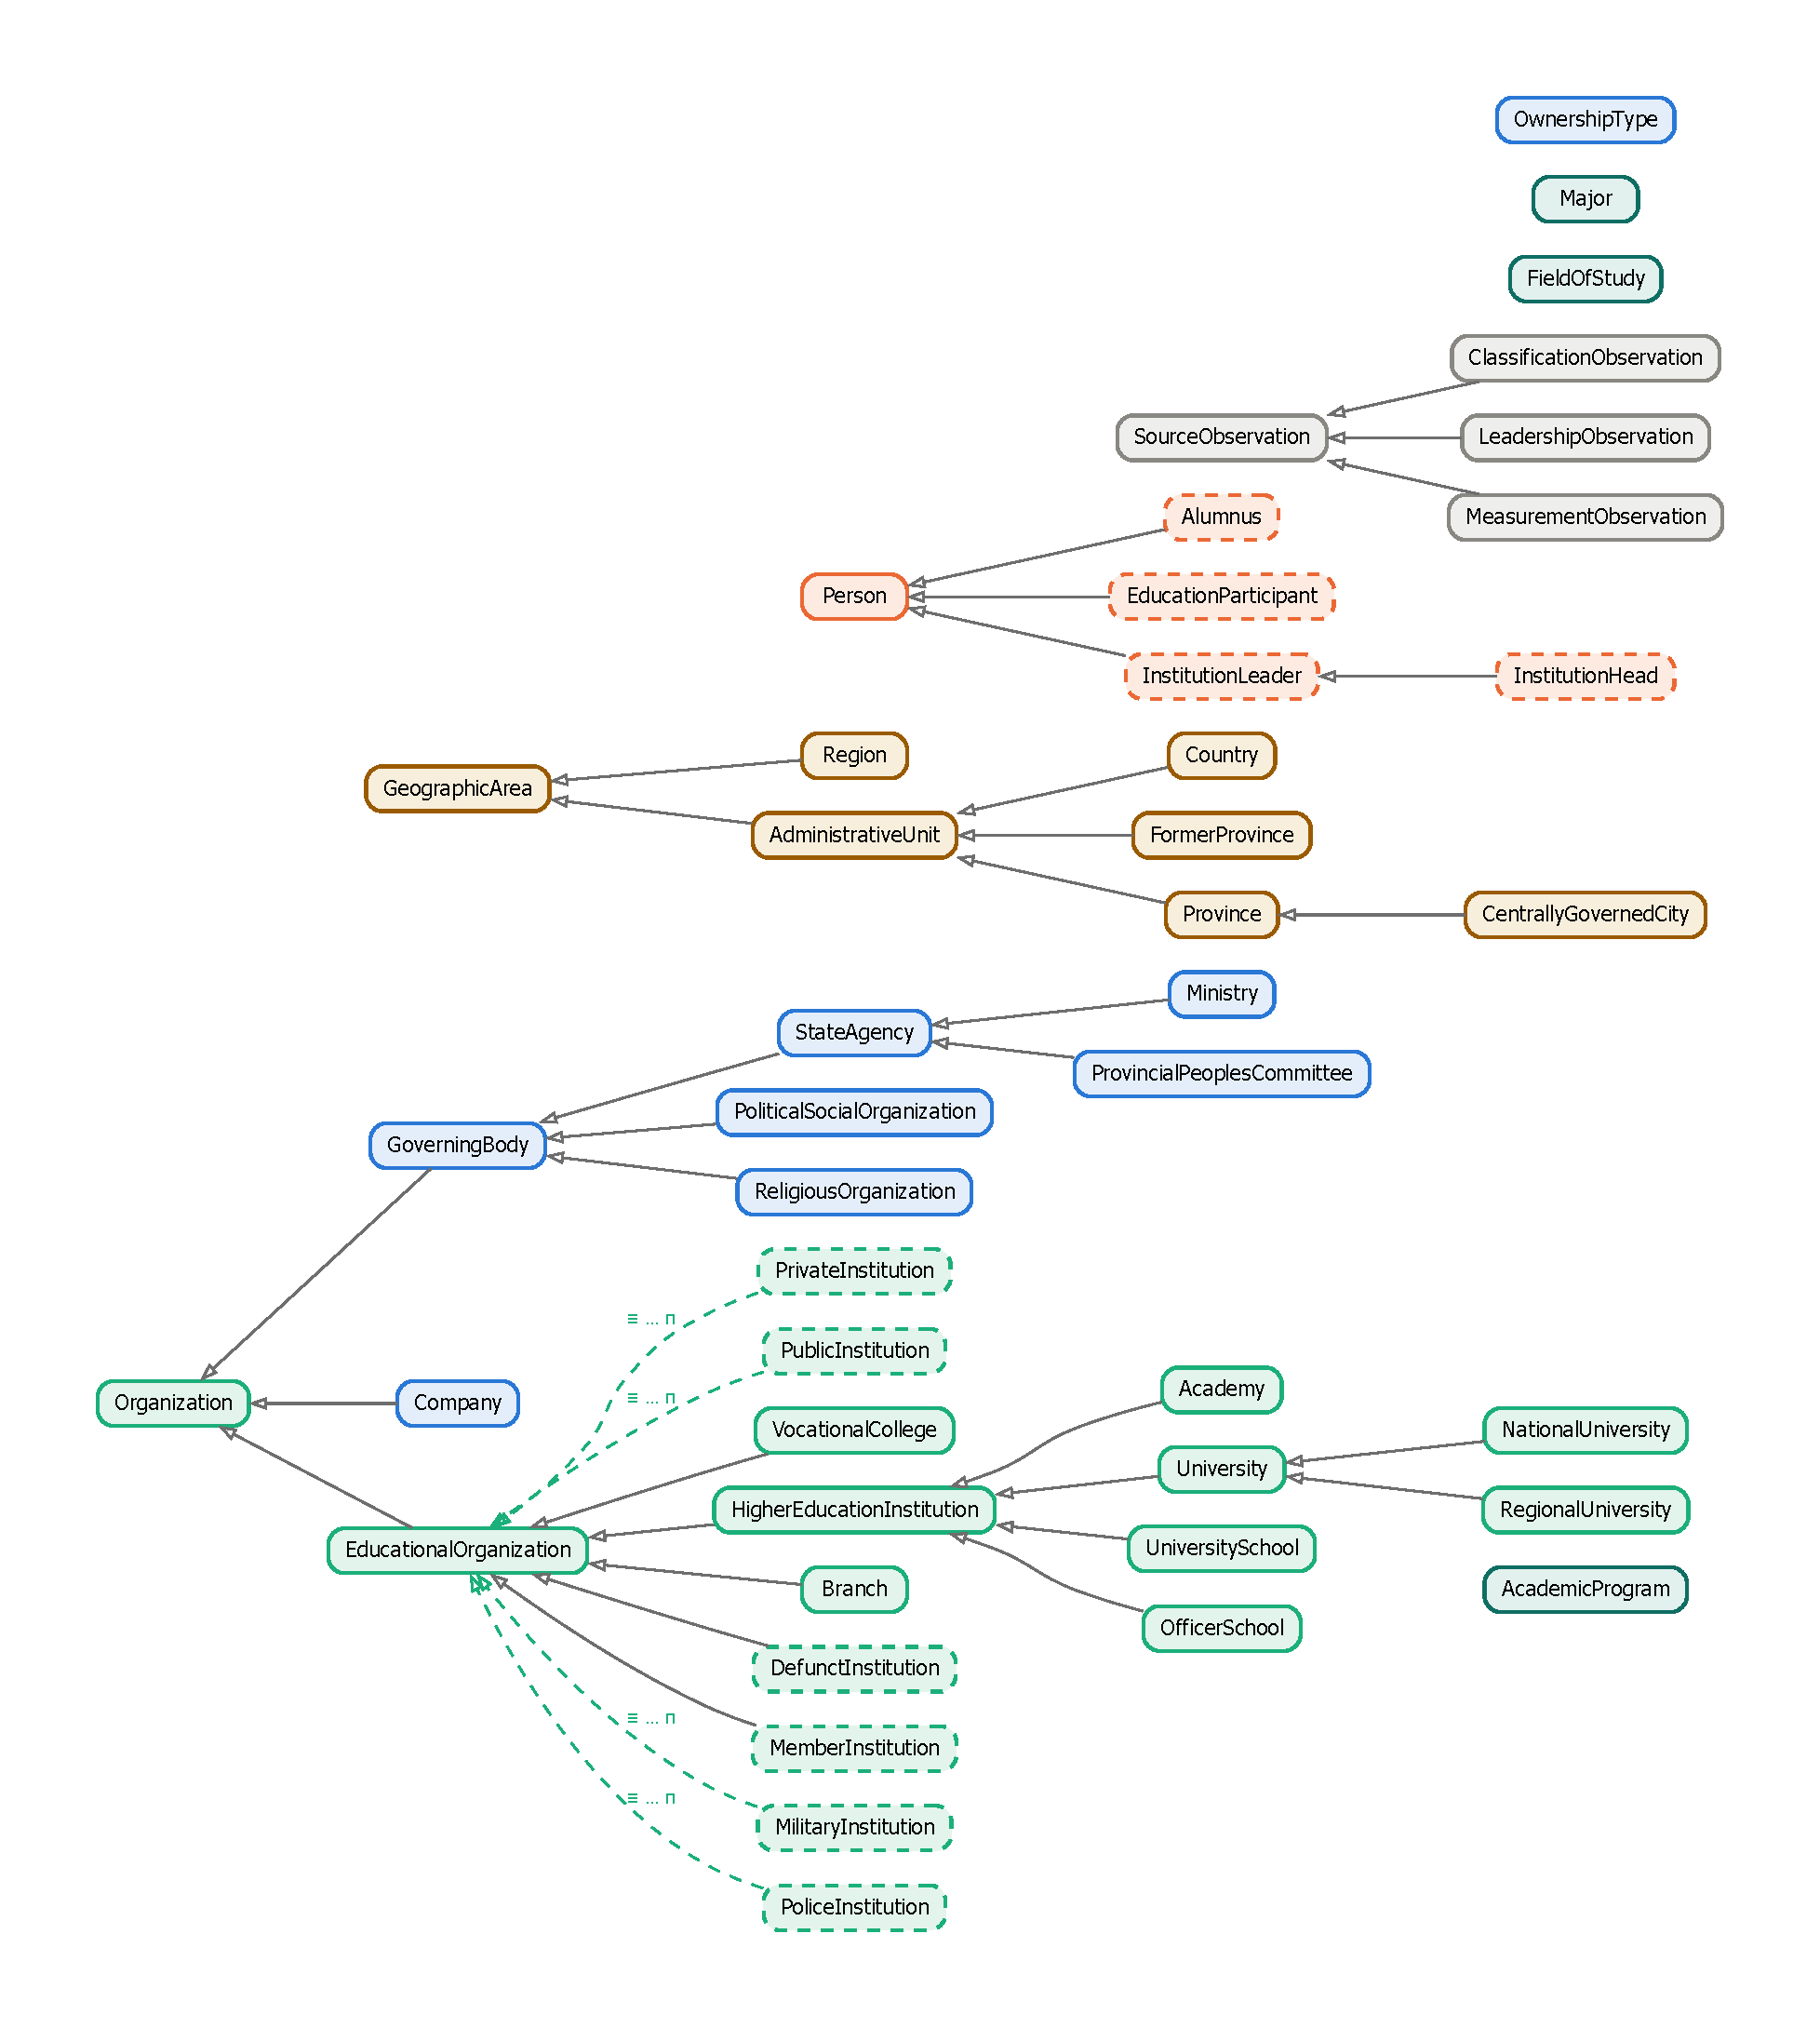
\includegraphics[height=0.6\textheight,width=\textwidth,keepaspectratio]{figures/gen/ontology-hierarchy.pdf}
\caption{Phân cấp lớp của ontology \texttt{vnedu:} 2.4, sinh tự động từ tệp ontology. Viền đứt: lớp định nghĩa bằng
\texttt{owl:equivalentClass}; màu: mô-đun.}\label{fig:hierarchy}
\end{figure}

\begin{figure}[htbp]
\centering
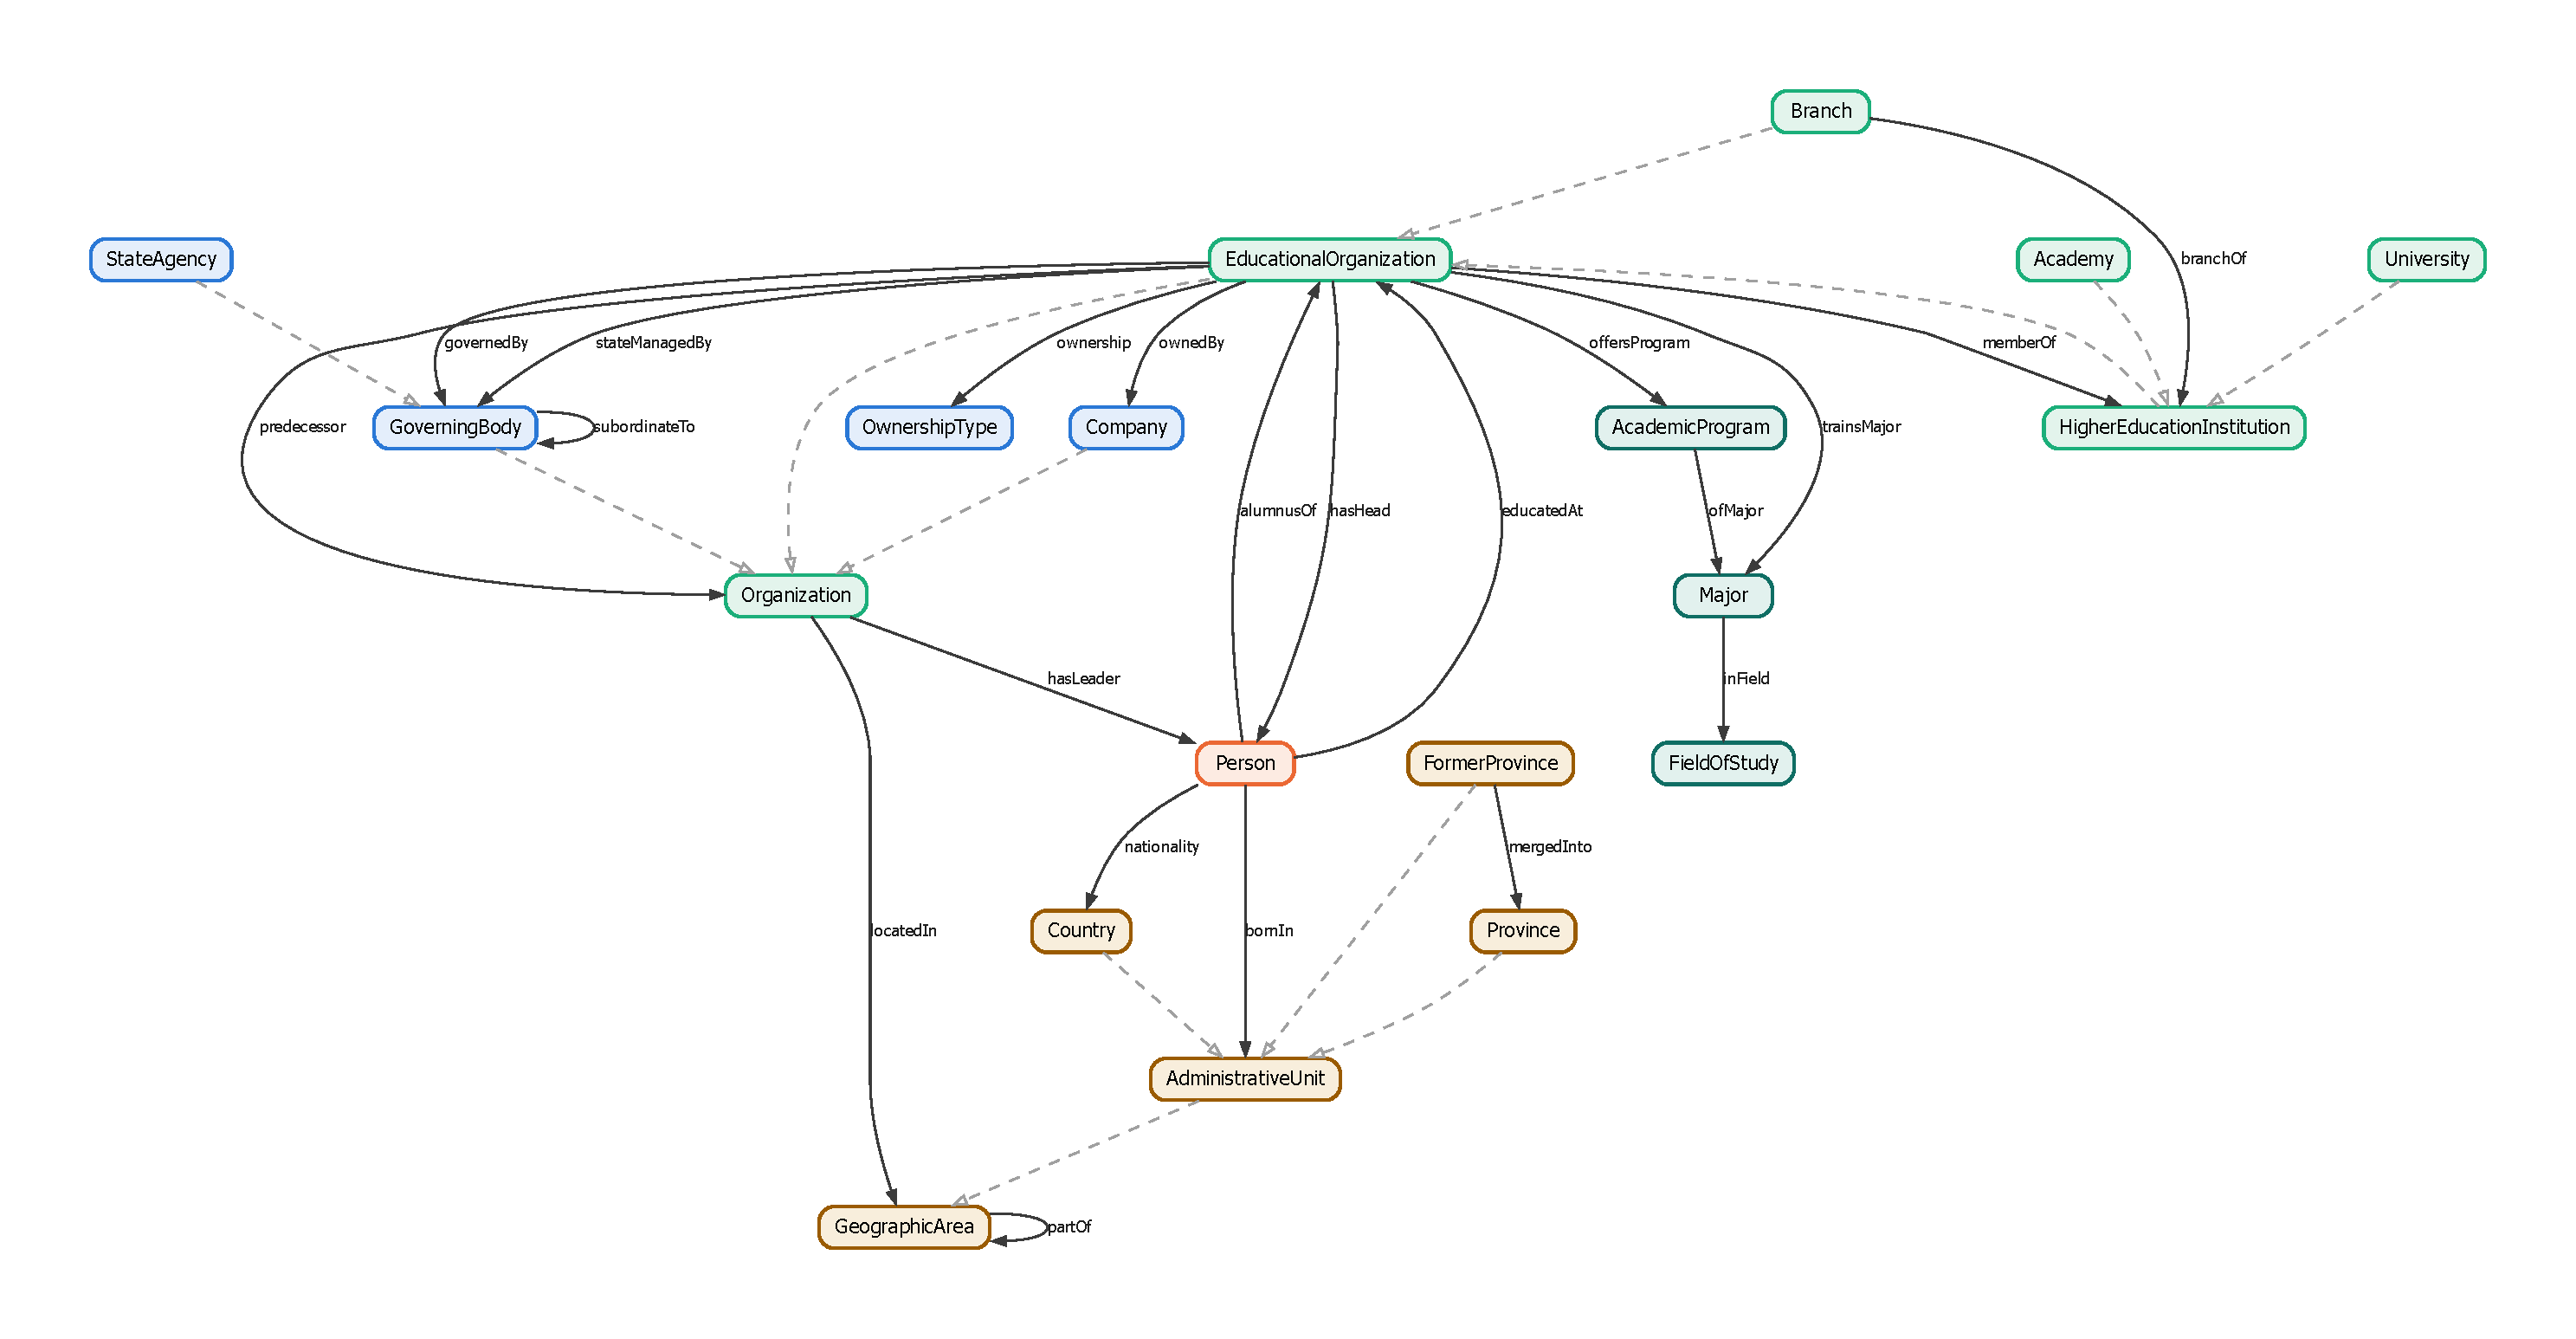
\includegraphics[width=\textwidth]{figures/gen/ontology-relations.pdf}
\caption{Quan hệ giữa các lớp. Cạnh liền: thuộc tính đối tượng (miền \(\to\) miền giá trị); cạnh đứt:
\texttt{rdfs:subClassOf}. Thuộc tính nghịch đảo và thuộc tính con được lược bớt.}\label{fig:relations}
\end{figure}

\subsection{Tiên đề suy luận}
\paragraph{Lớp định nghĩa.} Các lớp như cơ sở quân đội, công an, công lập, tư thục được định nghĩa bằng điều kiện cần và
đủ, nên bộ suy luận tự phân loại cá thể:
\begin{code}
vnedu:MilitaryInstitution owl:equivalentClass [
    owl:intersectionOf ( vnedu:EducationalOrganization
        [ a owl:Restriction ; owl:onProperty vnedu:governedBy ;
          owl:hasValue vnedu:MinistryOfNationalDefence ] ) ] .
vnedu:PrivateInstitution owl:equivalentClass [
    owl:intersectionOf ( vnedu:EducationalOrganization
        [ a owl:Restriction ; owl:onProperty vnedu:ownership ;
          owl:hasValue vnedu:PrivateOwnership ] ) ] ;
    owl:disjointWith vnedu:PublicInstitution .
\end{code}

\paragraph{Chuỗi thuộc tính.} \vn{partOf} là thuộc tính bắc cầu; bốn chuỗi \texttt{owl:propertyChainAxiom} lan truyền
địa điểm, chủ quản và ngành:
\begin{align*}
\textit{locatedIn} \circ \textit{mergedInto} &\sqsubseteq \textit{locatedIn} && \text{tỉnh cũ \(\to\) tỉnh mới}\\
\textit{locatedIn} \circ \textit{partOf} &\sqsubseteq \textit{locatedIn} && \text{tỉnh \(\to\) miền \(\to\) quốc gia}\\
\textit{governedBy} \circ \textit{subordinateTo} &\sqsubseteq \textit{governedBy} && \text{đơn vị trực thuộc \(\to\) Bộ}\\
\textit{offersProgram} \circ \textit{ofMajor} &\sqsubseteq \textit{trainsMajor} && \text{chương trình \(\to\) ngành}
\end{align*}
Chuỗi thứ nhất cho phép thống kê theo 34 tỉnh mới mà không sửa địa chỉ gốc; chuỗi thứ ba giúp phân loại đúng các trường
do một tổng cục hay quân chủng quản lý. Ontology còn có các cặp nghịch đảo (\vn{memberOf}/\vn{hasMember}), thuộc tính hàm
(\vn{foundingYear}, \vn{ownership}) và các nhóm lớp rời nhau để phát hiện dữ liệu mâu thuẫn.

\subsection{Nguồn gốc và thời gian}
Phần lớn nguồn chỉ cho biết ai giữ chức vụ tại thời điểm thu thập, không cho biết nhiệm kỳ. Vì vậy, các khẳng định phụ
thuộc thời gian (lãnh đạo, số liệu, phân loại) được ghi kèm một \vn{SourceObservation} (\texttt{prov:Entity}~\cite{w3c2013provo})
theo mẫu reification. Mỗi quan sát chứa nguồn, mã băm ảnh chụp nguồn, trạng thái thời gian và khoảng hiệu lực nếu biết.
Đồ thị có \metricObservations{} quan sát; trong đó chỉ 46 quan sát có thông tin thời gian, số còn lại mang trạng thái
\texttt{unknown}.

\subsection{Kiểm tra bằng công cụ}
Ontology được mở và kiểm tra trong Protégé 5.6.7~\cite{musen2015protege} (\cref{fig:protege}). Bộ kiểm tra hồ sơ của OWL
API~\cite{horridge2011owlapi} báo 0 vi phạm OWL~2~RL và OWL~2~DL (761 tiên đề). HermiT 1.4.3~\cite{glimm2014hermit} xác
nhận ontology nhất quán và không có lớp không thoả mãn được, kể cả khi nạp thêm TBox DBpedia (34{,}544 triple) để kiểm
tra các tiên đề căn chỉnh.

\IfFileExists{figures/protege-hermit.png}{%
\begin{figure}[htbp]
\centering
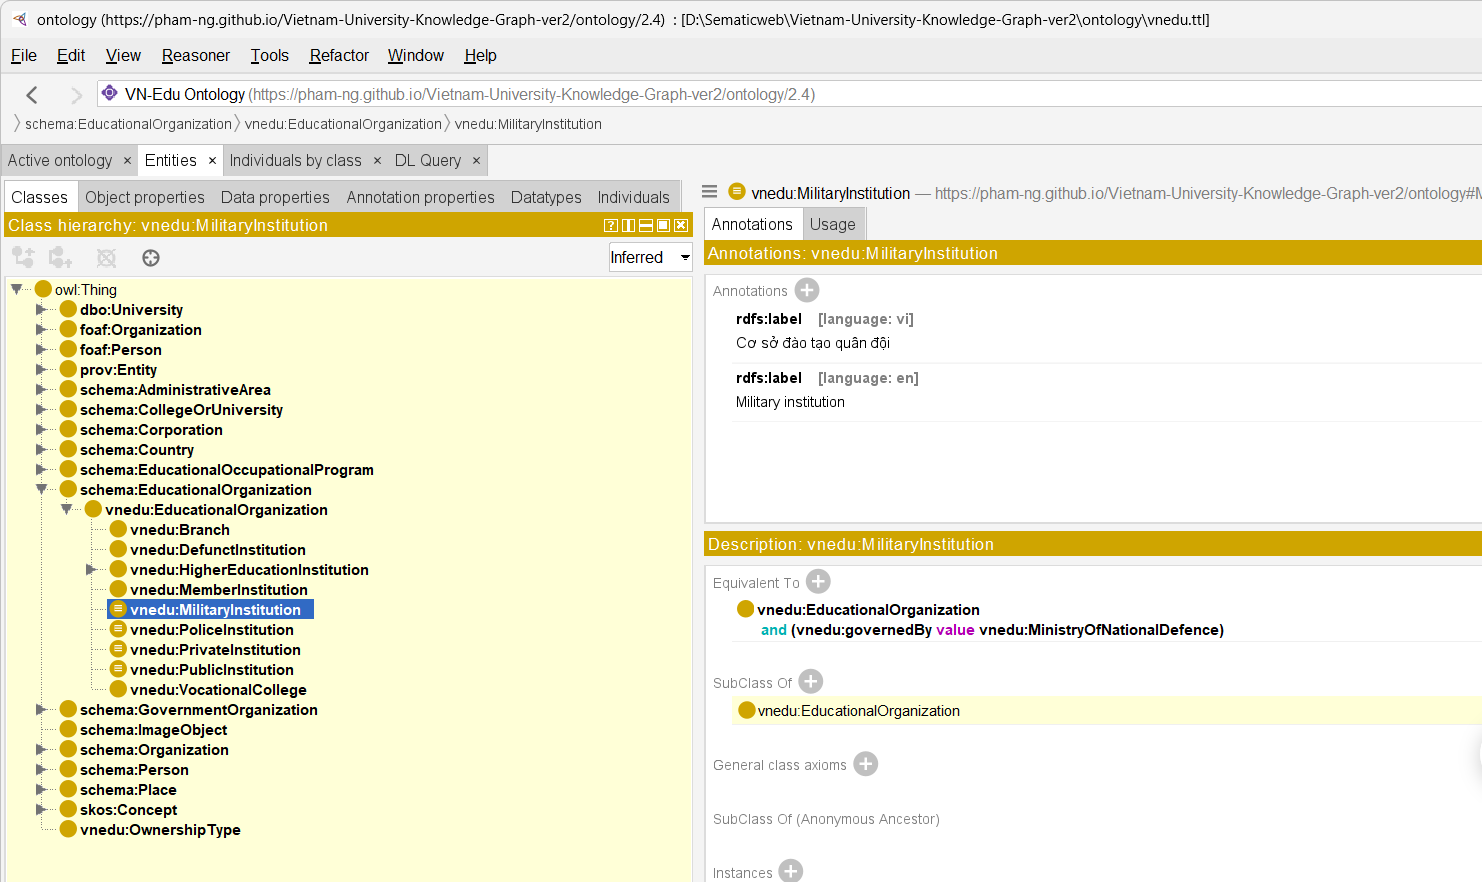
\includegraphics[width=\textwidth]{figures/protege-hermit.png}
\caption{Ontology \texttt{vnedu:} 2.4 trong Protégé 5.6.7 sau khi chạy HermiT 1.4.3. Trái: phân cấp lớp suy luận; các
lớp có biểu tượng \(\equiv\) là lớp định nghĩa. Phải: tiên đề tương đương của \texttt{vnedu:MilitaryInstitution}.}\label{fig:protege}
\end{figure}}{}

% ================================================================= 4
\section{Thu thập dữ liệu}\label{sec:collect}

\subsection{Nguồn dữ liệu}
\Cref{tab:sources} liệt kê các nguồn, giấy phép và số bản ghi thu được. Toàn bộ dữ liệu là ảnh chụp ngày 09/10/2026. Mỗi
tệp ở tầng Bronze có một tệp \texttt{.meta.json} ghi URL nguồn, thời điểm thu thập, giấy phép và mã băm. Mọi phản hồi HTTP
được lưu trong \texttt{data/bronze/http\_cache.zip}, nên có thể dựng lại dữ liệu mà không cần truy cập mạng.

\begin{table}[htbp]
\centering\small
\caption{Nguồn dữ liệu (ảnh chụp 09/10/2026).}\label{tab:sources}
\begin{tabularx}{\textwidth}{>{\raggedright\arraybackslash}p{3.1cm}>{\raggedright\arraybackslash}p{2.4cm}r>{\raggedright\arraybackslash}X}
\toprule
Nguồn (truy cập) & Giấy phép & Bản ghi & Dùng cho \\
\midrule
Wikidata (SPARQL) & CC0 1.0 & 363 & Cơ sở, định danh, ROR/GeoNames, toạ độ \\
& & 1{,}531 & Người có quan hệ học tập (\texttt{P69}) \\
& & 63 & Tỉnh, thành phố \\
Wikipedia tiếng Việt (MediaWiki API) & CC BY-SA 4.0 & 279 & Infobox (mã trường, chủ quản), tóm tắt, lịch sử \\
Cổng tuyển sinh Bộ GD\&ĐT & Không công bố giấy phép mở & 405 & Mã tuyển sinh, tên, địa chỉ \\
ROR (REST API) & CC0 1.0 & 202 & Định danh tổ chức nghiên cứu \\
DBpedia (SPARQL) & CC BY-SA 3.0 & 72 & Năm thành lập dự phòng, liên kết \\
OpenStreetMap (Nominatim) & ODbL 1.0 & 126 triple & Toạ độ bổ sung, tách thành tệp riêng \\
Bảng tham chiếu & Văn bản pháp luật & -- & Sáp nhập tỉnh 2025, miền, chủ quản theo quyết định, danh mục ngành
(TT~09/2022~\cite{vn2022tt09}) \\
\bottomrule
\end{tabularx}
\end{table}

\paragraph{Giấy phép.} Phần biên soạn của nhóm (ontology, mô hình dữ liệu, liên kết) được phát hành theo CC~BY-SA~4.0,
tương thích với điều kiện share-alike của Wikipedia. Giấy phép này không tái cấp phép nội dung của bên thứ ba: toạ độ từ
OpenStreetMap được tách thành tệp riêng theo ODbL; dữ liệu từ cổng tuyển sinh chỉ gồm các sự kiện công khai tối thiểu và
luôn kèm nguồn, vì cổng này không công bố giấy phép dữ liệu mở.

\subsection{Tích hợp}
Bản ghi được hợp nhất theo QID Wikidata, mã tuyển sinh và tên đã chuẩn hoá, rồi kiểm tra bằng JSON Schema. Mỗi giá trị
kèm \texttt{field\_sources} ghi nguồn của nó. Khi các nguồn mâu thuẫn, giá trị được chọn theo thứ tự ưu tiên: văn bản
pháp lý, Bộ GD\&ĐT, Wikidata, Wikipedia, DBpedia; các giá trị còn lại được ghi vào nhật ký xung đột. Năm ``truyền thống''
(tính từ đơn vị tiền thân) được tách khỏi năm thành lập theo quyết định (\vn{establishmentYear}). Quan hệ
\vn{directlyGovernedBy} chỉ được gán khi có văn bản pháp lý, còn quan hệ chủ quản do nguồn cộng đồng ghi nhận được lưu
riêng là \vn{reportedGovernedBy}.

\subsection{Thống kê bộ dữ liệu}
\Cref{tab:stats} tóm tắt bản phát hành. Độ phủ của các thuộc tính chính trên \metricInstitutions{} cơ sở: tỉnh/thành
96\%, năm thành lập 93\%, website 87\%, loại hình sở hữu 86\%, mã tuyển sinh 74\%, toạ độ 59\%, quy mô sinh viên 9\%. Bộ dữ
liệu chỉ gồm các cơ sở được mô tả trong những nguồn trên, và không phải danh mục chính thức của nhà nước.

\begin{table}[htbp]
\centering\small
\caption{Thống kê bản phát hành (sinh tự động bởi \texttt{audit/release\_metrics.py}).}\label{tab:stats}
\footnotesize\begin{tabular}{lr@{\hspace{0.6cm}}lr}
\toprule
Thực thể & Số lượng & Đồ thị con & Triple \\
\midrule
Cơ sở giáo dục & \metricInstitutions & Dữ liệu khẳng định & \metricAssertedTriples \\
\quad trong đó cơ sở GDĐH & \metricHEIs{} (258 đang hoạt động) & \quad trong đó siêu dữ liệu quan sát & 35{,}538 \\
Cá nhân & \metricPeople & Liên kết ra ngoài & \metricLinkTriples \\
\quad lãnh đạo / người từng học & \metricLeaders{} / \metricEducationParticipants & Suy luận OWL~2~RL & \metricInferredTriples \\
Cơ quan chủ quản & 50 & Toạ độ OSM (ODbL) & \metricOsmCoordinateTriples \\
Tỉnh mới / tỉnh cũ / miền & 34 / 29 / 3 & Ontology & \metricOntologyTriples \\
Ngành / lĩnh vực / chương trình mẫu & \metricMajors{} / 16 / \metricPrograms & VoID/DCAT & \metricMetadataTriples \\
URI cục bộ & \metricLocalResources & \textbf{Tổng} & \textbf{\metricUnionTriples} \\
\bottomrule
\end{tabular}
\end{table}

% ================================================================= 5
\section{Chuyển đổi sang dữ liệu 4 sao}\label{sec:transform}

\subsection{Pipeline Bronze--Silver--Gold}
Dữ liệu đi qua ba tầng (\cref{fig:medallion}): Bronze giữ nguyên phản hồi của nguồn, Silver là JSON đã chuẩn hoá và hợp
nhất, Gold là RDF cùng đồ thị liên kết và các triple suy luận. Trong thử nghiệm, hai lần dựng ngoại tuyến liên tiếp từ
bộ đệm cho ra các tệp Gold có cùng mã băm SHA-256.

\begin{figure}[htbp]
\centering
\resizebox{0.95\textwidth}{!}{%
\begin{tikzpicture}[node distance=1.5cm]
  \node[box=bronze, text width=4.1cm, minimum height=3.4cm, align=left] (B) {%
    \textbf{\large BRONZE}\\[2pt]\scriptsize
    \texttt{data/bronze/*.json}\\
    \texttt{*.meta.json}: nguồn, thời điểm, giấy phép\\
    \texttt{http\_cache.zip}: mọi phản hồi HTTP};
  \node[box=silver, text width=4.1cm, minimum height=3.4cm, align=left, right=of B] (S) {%
    \textbf{\large SILVER}\\[2pt]\scriptsize
    \texttt{institutions.json}, \texttt{people.json}, \texttt{uri\_map.json}\\
    hợp nhất, quy tỉnh cũ\(\to\)mới, nhật ký xung đột, JSON Schema};
  \node[box=gold, text width=4.1cm, minimum height=3.4cm, align=left, right=of S] (G) {%
    \textbf{\large GOLD}\\[2pt]\scriptsize
    \texttt{vnedu-data.ttl}, \texttt{vnedu-links.ttl}\\
    \texttt{vnedu-inferred.ttl}, \texttt{void.ttl}\\
    \texttt{vnedu-geo-osm.ttl} (ODbL)\\
    \(\Rightarrow\) \texttt{vnedu-all.ttl} (\metricUnionTriples{} triple)};
  \draw[flow] (B) -- node[above, font=\scriptsize]{bước 3} (S);
  \draw[flow] (S) -- node[above, font=\scriptsize]{bước 3b--5} (G);
\end{tikzpicture}}
\caption{Ba tầng dữ liệu và các tệp chính.}\label{fig:medallion}
\end{figure}

\subsection{URI và RDF}
Mỗi thực thể có một IRI HTTP tạo từ tên không dấu, ví dụ
\url{https://pham-ng.github.io/Vietnam-University-Knowledge-Graph-ver2/resource/university/dai-hoc-bach-khoa-ha-noi}.
IRI được lưu trong sổ đăng ký \texttt{uri\_map.json}, nên không đổi khi thực thể đổi tên. IRI không đuôi định danh sự vật;
IRI có đuôi \texttt{.ttl}/\texttt{.jsonld} định danh tài liệu mô tả nó. Nhãn có thẻ ngôn ngữ, literal có kiểu, và
\texttt{prov:wasDerivedFrom} ghi nguồn cụ thể (\cref{lst:hust}).

\codetitle{Mô tả RDF của ĐHBK Hà Nội (rút gọn)}\label{lst:hust}
\begin{code}
university:dai-hoc-bach-khoa-ha-noi a vnedu:University ;
    rdfs:label "Đại học Bách khoa Hà Nội"@vi ,
               "Hanoi University of Science and Technology"@en ;
    vnedu:shortName "HUST" ;           vnedu:admissionCode "BKA" ;
    vnedu:foundingYear 1956 ;          vnedu:ownership vnedu:PublicOwnership ;
    vnedu:directlyGovernedBy organization:bo-giao-duc-va-dao-tao ;  # QĐ 1723
    vnedu:locatedIn province:ha-noi ;
    prov:wasDerivedFrom wd:Q3075696 ,
        <https://vi.wikipedia.org/w/index.php?oldid=75604914> ,
        <https://congbao.chinhphu.vn/van-ban/quyet-dinh-so-1723-qd-ttg-45825/58191.htm> ;
    owl:sameAs wd:Q3075696 , <https://ror.org/04nyv3z04> ,
        dbr:Hanoi_University_of_Science_and_Technology .
\end{code}

\subsection{Suy luận và kiểm định}
owlrl áp dụng các luật OWL~2~RL lên ontology và dữ liệu khẳng định, sinh thêm \metricInferredTriples{} triple
(\cref{tab:inferred}). Các liên kết \texttt{owl:sameAs} ra ngoài không được đưa vào bước này, vì quy tắc \texttt{eq-rep}
sẽ sao chép mọi triple sang URI bên ngoài.

\begin{table}[htbp]
\centering\small
\caption{Số cá thể được phân loại bởi các lớp định nghĩa.}\label{tab:inferred}
\begin{tabular}{lrl}
\toprule
Lớp & Cá thể & Điều kiện \\
\midrule
\texttt{Public-} / \texttt{PrivateInstitution} & 219 / 35 & \texttt{ownership} công lập / tư thục \\
\vn{InstitutionHead} & 198 & \(\exists\,\texttt{headOf}.\texttt{EducationalOrganization}\) \\
\vn{MemberInstitution} & 46 & \(\exists\,\texttt{memberOf}\) \\
\vn{MilitaryInstitution} & 21 & \texttt{governedBy} Bộ Quốc phòng (kể cả qua chuỗi) \\
\vn{DefunctInstitution} & 10 & \(\exists\,\texttt{dissolutionYear}\) \\
\vn{PoliceInstitution} & 7 & \texttt{governedBy} Bộ Công an \\
\bottomrule
\end{tabular}
\end{table}

Sau đó, các shape SHACL~\cite{w3c2017shacl} kiểm tra đồ thị: mã tuyển sinh gồm 3 chữ in hoa, toạ độ nằm trong lãnh thổ
Việt Nam, năm thành lập không sau năm giải thể, cơ sở tư thục không có Bộ làm chủ quản, v.v. Kết quả gồm 0 vi phạm,
\metricWarnings{} cảnh báo về giá trị tuỳ chọn còn thiếu (21 cơ sở thiếu năm thành lập, 12 thiếu tỉnh) và
\metricInformationResults{} kết quả thông tin. Bản phát hành chỉ được công bố khi các kiểm tra đều đạt. Với các thực thể
có IRI HTTP tra cứu được, dữ liệu đáp ứng mức 4 sao.

% ================================================================= 6
\section{Liên kết: dữ liệu 5 sao}\label{sec:link}

\subsection{Liên kết ra ngoài}
Đồ thị liên kết gồm \metricLinkTriples{} triple: 2{,}310 \texttt{owl:sameAs} (Wikidata 1{,}850, DBpedia 202, ROR 195,
GeoNames 63), 61 \texttt{skos:closeMatch} cho ngành và lĩnh vực, và \texttt{foaf:isPrimaryTopicOf} tới bài Wikipedia.
Liên kết định danh được lấy từ \emph{định danh dùng chung}, không từ so khớp tên:
\begin{itemize}
  \item QID Wikidata lấy từ chính bản ghi nguồn; ROR và GeoNames lấy từ thuộc tính \texttt{P6782} và \texttt{P1566} của
  Wikidata.
  \item DBpedia được tìm qua \texttt{?d owl:sameAs wd:Q…}, rồi đối chiếu với bài Wikipedia tiếng Anh mà Wikidata trỏ tới;
  chỉ giữ ánh xạ một--một. Bước này đã loại một số liên kết sai có sẵn trong DBpedia, chẳng hạn ĐHBK TP.HCM bị gắn vào
  ĐH Sư phạm Kỹ thuật TP.HCM.
  \item Ngành dùng \texttt{skos:closeMatch} thay vì \texttt{owl:sameAs}, vì khái niệm ngành trong danh mục Việt Nam
  không trùng hoàn toàn với khái niệm trên Wikidata~\cite{halpin2010sameas}.
\end{itemize}
Bộ dữ liệu được mô tả bằng VoID~\cite{w3c2011void} và DCAT~\cite{w3c2020dcat} (giấy phép, endpoint, các
\texttt{void:Linkset}).

\subsection{Thí nghiệm so khớp nhãn bằng Silk}
Để xem so khớp nhãn tự động hoạt động thế nào, chúng tôi chạy Silk 3.6.0~\cite{volz2009silk} (khoảng cách Levenshtein)
và một baseline Jaccard trên 86 cơ sở có nhãn tiếng Anh và 86 đích DBpedia (7{,}396 cặp ứng viên). Tập tham chiếu là các
liên kết sinh từ định danh, không phải tập gán nhãn độc lập; vì vậy \cref{tab:silk} đo \emph{mức đồng thuận} với liên
kết theo định danh, không đo độ chính xác tuyệt đối.

\begin{table}[htbp]
\centering\small
\caption{Mức đồng thuận của so khớp nhãn với liên kết theo định danh (86 cơ sở).}\label{tab:silk}
\begin{tabular}{lrrrr}
\toprule
Quy tắc & Dự đoán & Precision & Recall & F1 \\
\midrule
Silk, khoảng cách tối đa 0 & 57 & 100,0\% & 66,3\% & 0,797 \\
Silk, khoảng cách tối đa 3 & 64 & 98,4\% & 73,3\% & 0,840 \\
Silk, khoảng cách tối đa 8 & 75 & 93,3\% & 81,4\% & 0,870 \\
Jaccard \(\geq 0{,}4\) & 80 & 90,0\% & 83,7\% & 0,867 \\
Jaccard \(\geq 0{,}8\) & 68 & 94,1\% & 74,4\% & 0,831 \\
\bottomrule
\end{tabular}
\end{table}

Ngưỡng càng chặt thì precision càng cao và recall càng thấp; F1 cao nhất khoảng 0,87. Phân tích các trường hợp bất đồng
cho thấy những lỗi điển hình của so khớp nhãn. Ví dụ, ``Hanoi University of Science and Technology'' (ĐHBK Hà Nội) và
``University of Science and Technology of Hanoi'' (USTH) có cùng tập từ nên Jaccard cho điểm 1,00; trường thành viên cũng
thường bị khớp nhầm với đại học mẹ. Vì vậy, kết quả từ Silk chỉ dùng để tham khảo và không được đưa vào đồ thị công bố.

\subsection{Độ chính xác của liên kết đã công bố}
Để ước lượng độ chính xác, chúng tôi rút ngẫu nhiên phân tầng 100 liên kết \texttt{owl:sameAs} (seed cố định). Mỗi liên
kết được đối chiếu với siêu dữ liệu của trang đích: loại thực thể phải tương thích (\texttt{P31} của Wikidata,
\texttt{rdf:type} của DBpedia, loại ROR, \texttt{featureCode} của GeoNames), tên phải khớp, và với người thì năm sinh phải
trùng. Có 93 liên kết qua kiểm tra tự động; 7 liên kết còn lại được một thành viên đánh giá thủ công, có ghi bằng chứng.
Không phát hiện liên kết sai nào (\cref{tab:precision}). Khoảng tin cậy Wilson~\cite{wilson1927} được dùng vì khoảng Wald
suy biến khi \(\hat p = 1\). Hai lưu ý: kiểm tra tự động và bộ liên kết cùng dựa phần nào vào nhãn tên nên không hoàn toàn
độc lập; và phương pháp này chỉ ước lượng precision, không ước lượng recall. Với liên kết tới bốn bộ dữ liệu ngoài, dữ liệu
đáp ứng mức 5 sao.

\begin{table}[htbp]
\centering\small
\caption{Kết quả kiểm tra \texttt{owl:sameAs} trên mẫu ngẫu nhiên phân tầng.}\label{tab:precision}
\begin{tabular}{lrrrl}
\toprule
Tầng & Liên kết & Mẫu & Đúng & Wilson 95\% \\
\midrule
Wikidata & 1{,}850 & 60 & 60 & 94,0--100\% \\
DBpedia & 202 & 20 & 20 & 83,9--100\% \\
ROR & 195 & 10 & 10 & 72,2--100\% \\
GeoNames & 63 & 10 & 10 & 72,2--100\% \\
\midrule
\textbf{Tổng} & 2{,}310 & 100 & 100 & \textbf{96,3--100\%} \\
\bottomrule
\end{tabular}
\end{table}

% ================================================================= 7
\section{SPARQL endpoint và ứng dụng web}\label{sec:publish}

\subsection{Trang Linked Data và ứng dụng web}
Mỗi thực thể có một trang HTML (nhúng JSON-LD, có \texttt{<link rel="alternate">} trỏ tới bản RDF), một tệp Turtle và
một tệp JSON-LD. Trên Render, cùng một IRI trả về HTML hoặc RDF tuỳ theo tiêu đề \texttt{Accept}, kèm
\texttt{Vary: Accept}. Khuyến nghị Cool URIs~\cite{w3c2008cooluris} là dùng chuyển hướng 303; do GitHub Pages không hỗ
trợ 303, chúng tôi trả biểu diễn trực tiếp và công bố URI tài liệu riêng có đuôi, để hai kênh có cùng hành vi.

\Cref{fig:web} trình bày một số màn hình của ứng dụng web. Trang tài nguyên hiển thị hộp thông tin kiểu Wikipedia, trong
đó mỗi giá trị kèm nguồn và các liên kết ra ngoài. Trang SPARQL có sẵn các truy vấn mẫu. Trên trang tĩnh, toàn bộ đồ thị
(khoảng 5~MB) được nạp vào Oxigraph/WASM trong khoảng 0,24~giây, nên truy vấn chạy ngay trên máy người dùng.

\begin{figure}[htbp]
\centering
\begin{subfigure}[t]{0.49\textwidth}\centering
  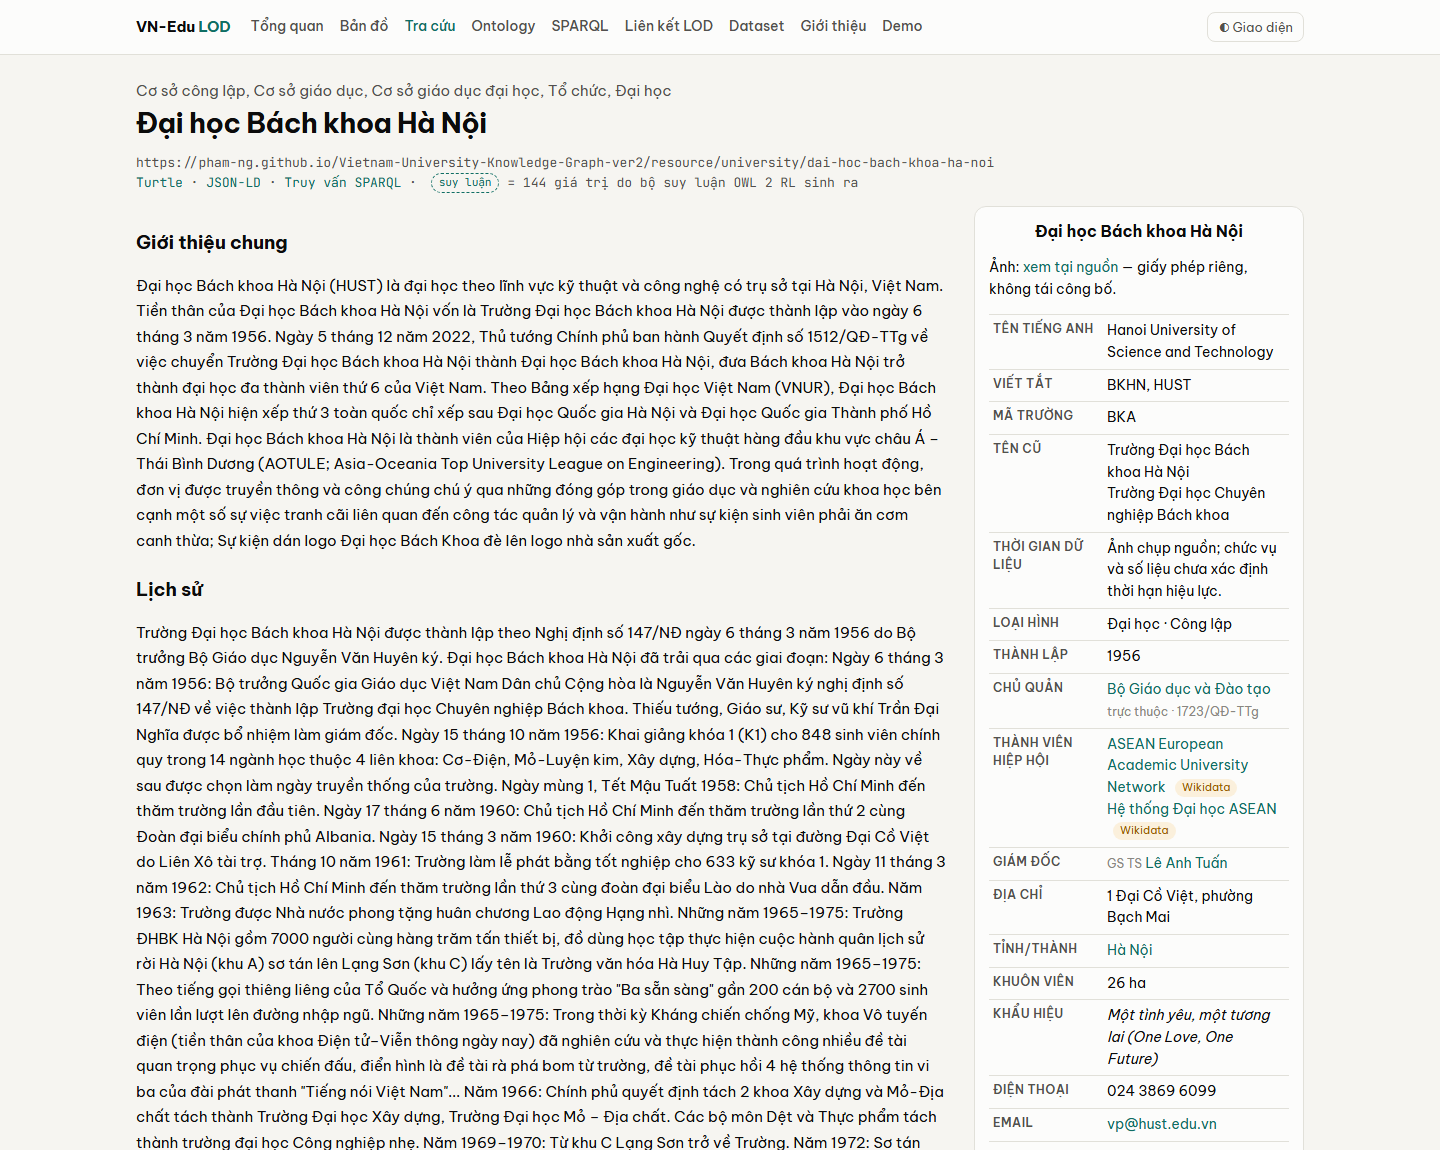
\includegraphics[width=\textwidth]{figures/gen/web-hust.png}\caption{Trang tài nguyên ĐHBK Hà Nội}\end{subfigure}\hfill
\begin{subfigure}[t]{0.49\textwidth}\centering
  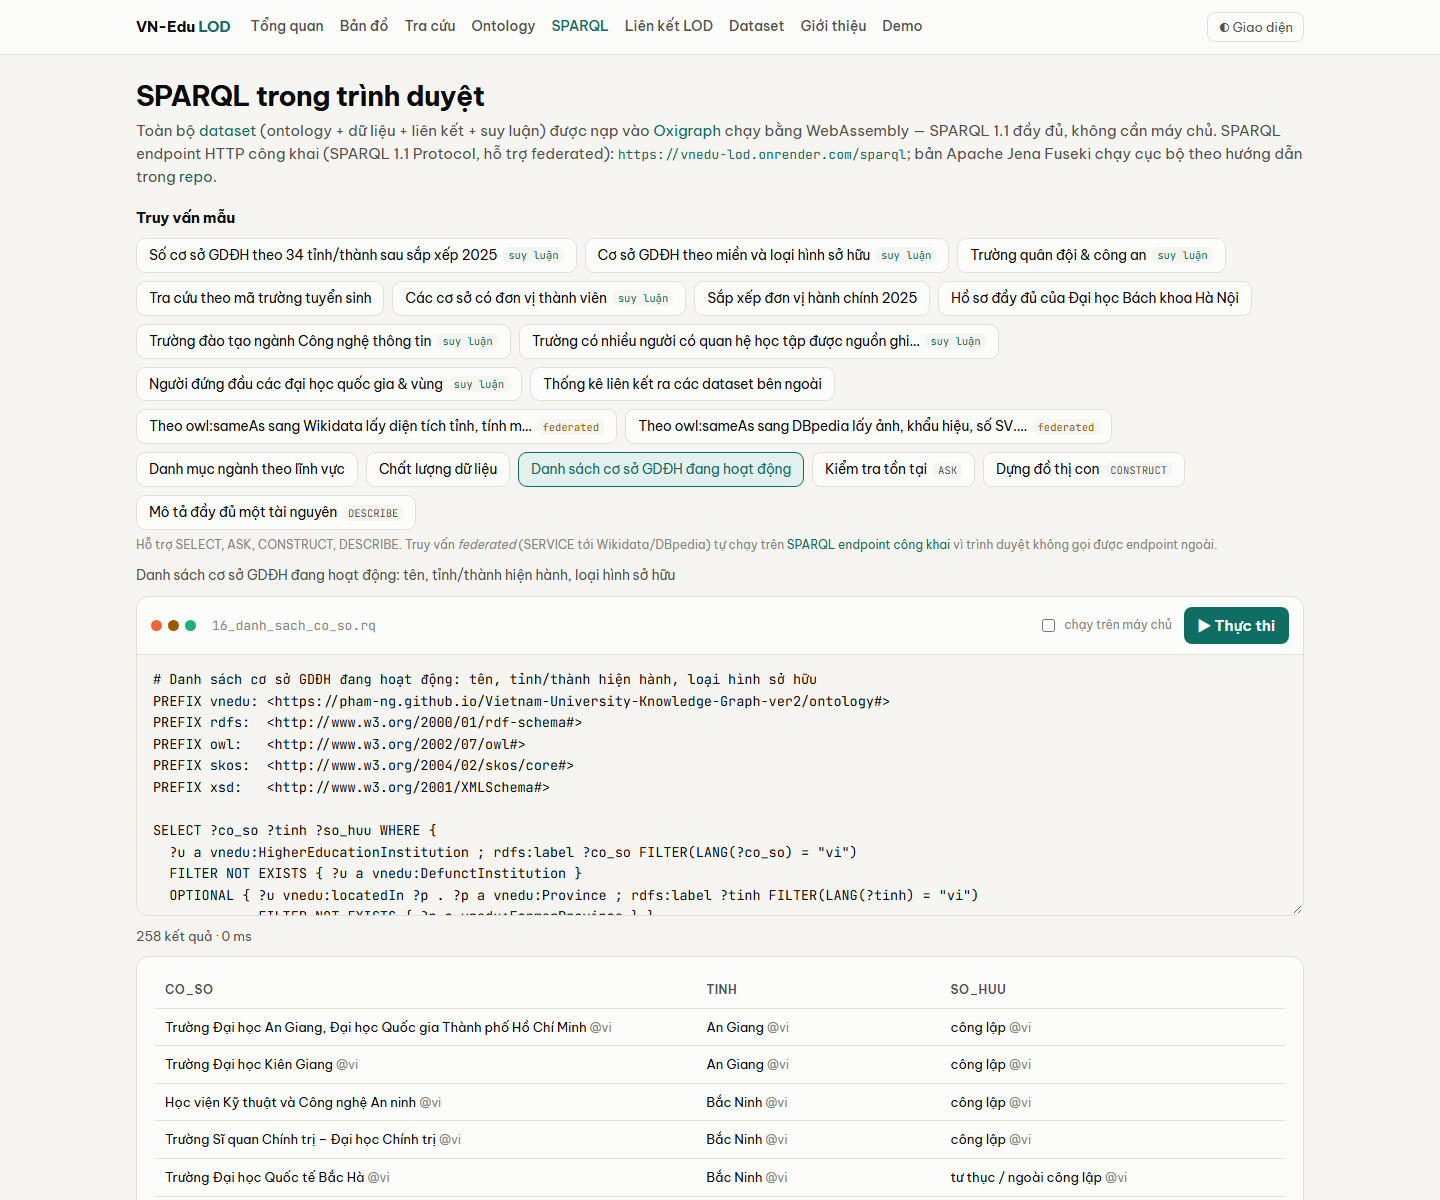
\includegraphics[width=\textwidth]{figures/gen/web-sparql.png}\caption{Trình soạn SPARQL và truy vấn mẫu}\end{subfigure}
\\[6pt]
\begin{subfigure}[t]{0.49\textwidth}\centering
  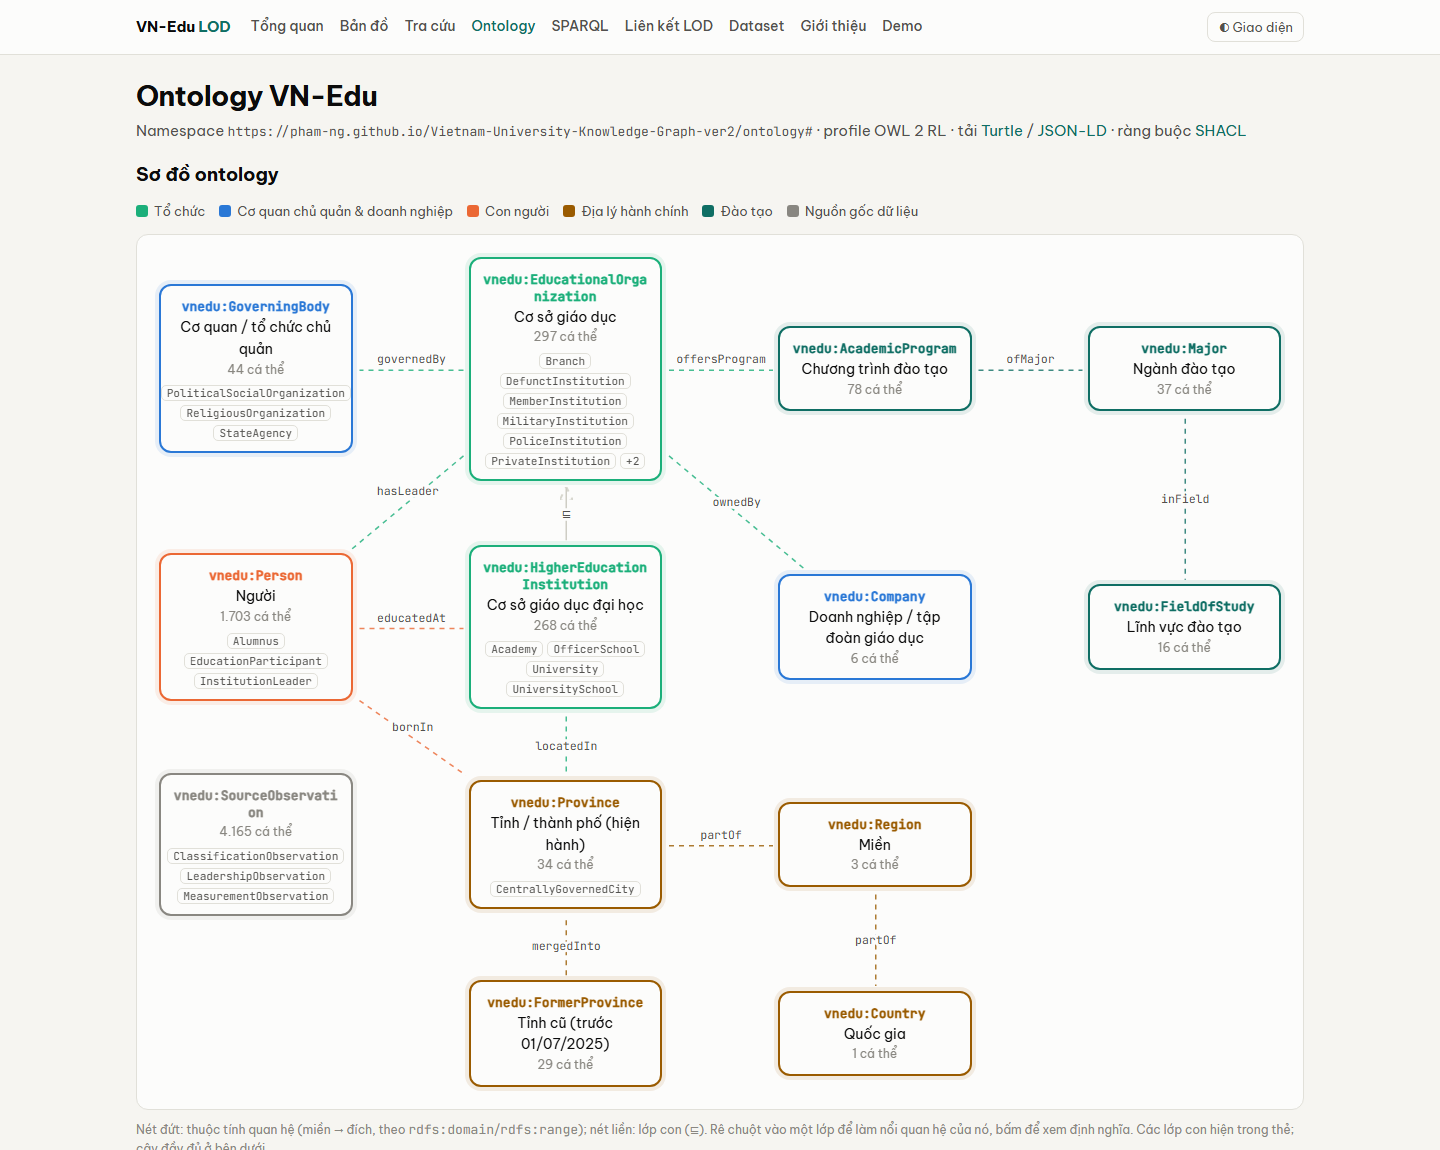
\includegraphics[width=\textwidth]{figures/gen/web-ontology.png}\caption{Sơ đồ ontology}\end{subfigure}\hfill
\begin{subfigure}[t]{0.49\textwidth}\centering
  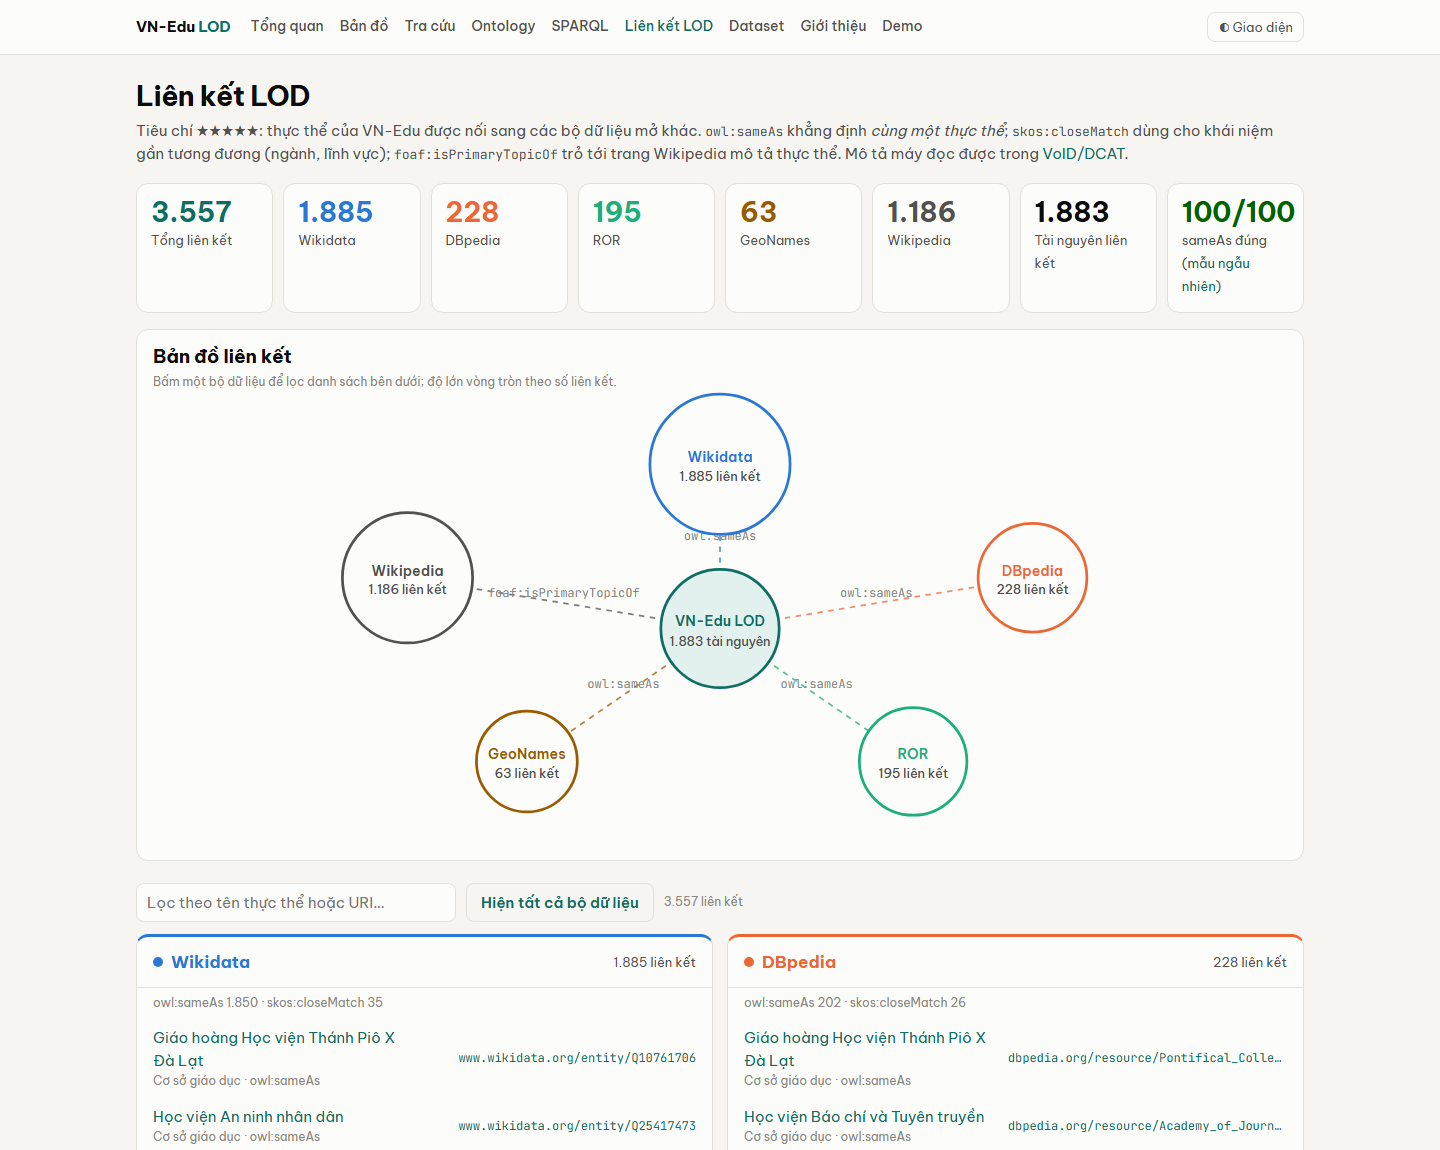
\includegraphics[width=\textwidth]{figures/gen/web-links.png}\caption{Các linkset ra ngoài}\end{subfigure}
\caption{Một số màn hình của ứng dụng web VN-Edu LOD.}\label{fig:web}
\end{figure}

\subsection{SPARQL endpoint}
Endpoint \texttt{/sparql} tuân thủ giao thức SPARQL~1.1~\cite{w3c2013sparql}, trả kết quả dạng JSON, CSV, TSV, XML,
Turtle hoặc JSON-LD, và trả \texttt{406} nếu định dạng yêu cầu không được hỗ trợ. Endpoint chỉ cho đọc: \texttt{UPDATE}
và \texttt{FROM} bị chặn; \texttt{SERVICE} chỉ được gọi tới Wikidata và DBpedia; mỗi truy vấn chạy trong tiến trình riêng
có giới hạn thời gian, và máy chủ trả \texttt{503} kèm \texttt{Retry-After} khi quá tải.

\subsection{Các truy vấn tiêu biểu}\label{sec:queries}
Kho mã có 19 truy vấn mẫu trong thư mục \texttt{queries/}. Dưới đây là năm truy vấn minh hoạ những gì đồ thị trả lời được
nhờ suy luận và liên kết. Kết quả được lấy từ bản phát hành hiện tại; khi chạy cục bộ, mỗi truy vấn mất dưới 1~giây.

\paragraph{(1) Phân bố theo miền và loại hình sở hữu.} Thông tin miền không được lưu trực tiếp mà được suy ra qua chuỗi
\(\textit{locatedIn}\circ\textit{partOf}\); cơ sở đã giải thể bị loại nhờ lớp suy ra \vn{DefunctInstitution}. Các cơ sở
chưa rõ loại hình sở hữu không được tính.
\begin{code}
SELECT ?mien ?loai (COUNT(DISTINCT ?u) AS ?n) WHERE {
  ?u a vnedu:HigherEducationInstitution ; vnedu:locatedIn ?r ;
     vnedu:ownership/rdfs:label ?loai .
  ?r a vnedu:Region ; rdfs:label ?mien .
  FILTER(LANG(?mien)="vi" && LANG(?loai)="vi")
  FILTER NOT EXISTS { ?u a vnedu:DefunctInstitution }
} GROUP BY ?mien ?loai
\end{code}
\begin{center}\small
\begin{tabular}{lrrr}
\toprule
Miền & Công lập & Tư thục & Tôn giáo \\
\midrule
Bắc Bộ & 112 & 10 & 1 \\
Trung Bộ & 37 & 6 & 0 \\
Nam Bộ & 54 & 16 & 0 \\
\bottomrule
\end{tabular}
\end{center}

\paragraph{(2) Cơ sở khối quân đội và công an.} Có 21 cơ sở quân đội và 7 cơ sở công an được phân loại tự động. Trong
21 cơ sở quân đội, 10 cơ sở được nguồn ghi là trực thuộc một đơn vị cấp dưới (Tổng cục Chính trị, Quân chủng Hải quân,
Binh chủng Pháo binh,\dots) và chỉ được xếp vào lớp này nhờ chuỗi \(\textit{governedBy}\circ\textit{subordinateTo}\).
\begin{code}
SELECT ?loai (COUNT(DISTINCT ?u) AS ?n)
       (COUNT(DISTINCT ?gian_tiep) AS ?qua_chuoi)
WHERE {
  VALUES (?c ?loai ?bo) {
    (vnedu:MilitaryInstitution "Quân đội" vnedu:MinistryOfNationalDefence)
    (vnedu:PoliceInstitution   "Công an"  vnedu:MinistryOfPublicSecurity) }
  ?u a ?c .
  OPTIONAL { ?u vnedu:governedBy ?b .
             ?b vnedu:subordinateTo+ ?bo .
             BIND(?u AS ?gian_tiep) }
} GROUP BY ?loai
\end{code}
\begin{center}\small
\begin{tabular}{lrr}
\toprule
\texttt{?loai} & \texttt{?n} & \texttt{?qua\_chuoi} \\
\midrule
Quân đội & 21 & 10 \\
Công an & 7 & 0 \\
\bottomrule
\end{tabular}
\end{center}

\paragraph{(3) Các trường thành viên của Đại học Quốc gia Hà Nội.} Dữ liệu chỉ ghi \vn{memberOf} ở phía trường thành
viên; quan hệ ngược \vn{hasMember} được suy ra. Truy vấn liệt kê các đơn vị thành viên cùng mã tuyển sinh và năm thành
lập. Với các đại học khác, số đơn vị thành viên trong dữ liệu là: ĐH Huế và ĐHQG TP.HCM mỗi đại học 8, ĐH Thái Nguyên 7,
ĐH Đà Nẵng 6.
\begin{code}
SELECT ?thanh_vien ?ma ?nam WHERE {
  ?dhqg rdfs:label "Đại học Quốc gia Hà Nội"@vi ; vnedu:hasMember ?tv .
  ?tv rdfs:label ?thanh_vien FILTER(LANG(?thanh_vien)="vi")
  OPTIONAL { ?tv vnedu:admissionCode ?ma }  OPTIONAL { ?tv vnedu:foundingYear ?nam }
} ORDER BY ?nam
\end{code}
\begin{center}\small
\begin{tabular}{lll@{\hspace{1cm}}lll}
\toprule
Đơn vị thành viên & Mã & Năm & Đơn vị thành viên & Mã & Năm \\
\midrule
Trường ĐH Khoa học Tự nhiên & QHT & 1904\textsuperscript{*} & Trường Quốc tế & QHQ & 2002 \\
Trường ĐH KHXH và Nhân văn & QHX & 1945 & Trường ĐH Công nghệ & QHI & 2004 \\
Trường ĐH Ngoại ngữ & QHF & 1955 & Trường ĐH Giáo dục & QHS & 2009 \\
Trường ĐH Kinh tế & QHE & 1974 & Trường ĐH Y Dược & QHY & 2010 \\
Trường ĐH Luật & QHL & 1976 & Trường ĐH Việt Nhật & VJU & 2016 \\
Trường Quản trị và Kinh doanh & QHD & 1995 & Viện Trần Nhân Tông & VVT & -- \\
Trường KH liên ngành và Nghệ thuật & QHK & 2002 & & & \\
\bottomrule
\end{tabular}
\par\smallskip\footnotesize\textsuperscript{*}Năm ``truyền thống'' theo nguồn, tính từ đơn vị tiền thân.
\end{center}

\paragraph{(4) Truy vấn liên hợp sang Wikidata: mật độ cơ sở theo tỉnh mới.} Truy vấn đếm số cơ sở theo 34 tỉnh mới (suy
ra qua \(\textit{locatedIn}\circ\textit{mergedInto}\)), đi theo \texttt{owl:sameAs} sang Wikidata để lấy diện tích
(\texttt{wdt:P2046}) bằng \texttt{SERVICE}~\cite{w3c2013sparqlfed}, rồi tính mật độ. Diện tích lấy trực tiếp từ Wikidata
tại thời điểm truy vấn.
\begin{code}
SELECT ?tinh ?so_co_so ?dien_tich_km2 ?mat_do WHERE {
  { SELECT ?wd ?tinh (COUNT(DISTINCT ?u) AS ?so_co_so) WHERE {
      ?u a vnedu:HigherEducationInstitution ; vnedu:locatedIn ?t .
      ?t a vnedu:Province ; rdfs:label ?tinh ; owl:sameAs ?wd .
      FILTER(LANG(?tinh)="vi"
             && STRSTARTS(STR(?wd), "http://www.wikidata.org/entity/"))
    } GROUP BY ?wd ?tinh ORDER BY DESC(?so_co_so) LIMIT 6 }
  OPTIONAL { SERVICE <https://query.wikidata.org/sparql> {
               ?wd wdt:P2046 ?dien_tich_km2 } }
  BIND(ROUND(100000 * ?so_co_so / ?dien_tich_km2) / 100 AS ?mat_do)
} ORDER BY DESC(?so_co_so)
\end{code}
\begin{center}\small
\begin{tabular}{lrrr}
\toprule
Tỉnh/thành (sau 2025) & Số cơ sở & Diện tích (km\(^2\), Wikidata) & Cơ sở / 1000 km\(^2\) \\
\midrule
Hà Nội & 101 & 3{,}360 & 30,06 \\
TP. Hồ Chí Minh & 58 & 6{,}773 & 8,56 \\
Huế & 13 & 4{,}947 & 2,63 \\
Đà Nẵng & 13 & 11{,}860 & 1,10 \\
Thái Nguyên & 8 & 8{,}375 & 0,96 \\
Khánh Hòa & 6 & 8{,}556 & 0,70 \\
\bottomrule
\end{tabular}
\end{center}

\paragraph{(5) Cơ sở có liên kết tới nhiều bộ dữ liệu.} Có 79 cơ sở GDĐH liên kết đồng thời tới Wikidata, DBpedia và ROR.
\begin{code}
SELECT (COUNT(DISTINCT ?u) AS ?n) WHERE {
  ?u a vnedu:HigherEducationInstitution ; owl:sameAs ?wd , ?db , ?ror .
  FILTER(STRSTARTS(STR(?wd), "http://www.wikidata.org/")
         && STRSTARTS(STR(?db), "http://dbpedia.org/")
         && STRSTARTS(STR(?ror), "https://ror.org/"))
}
\end{code}

\subsection{Apache Jena Fuseki}
Ngoài máy chủ rdflib, đồ thị được nạp vào Apache Jena Fuseki 6.2.0 với lưu trữ bền vững TDB2. Script
\texttt{audit/fuseki\_e2e.py} tự động hoá toàn bộ quy trình:
\begin{enumerate}
  \item Khởi động một Fuseki tạm (bản chính thức, đã kiểm tra SHA-512) ở chế độ cho phép ghi, chỉ lắng nghe trên
  \texttt{127.0.0.1}.
  \item Nạp \texttt{vnedu-all.ttl} qua giao thức Graph Store, kiểm tra việc ghi đè và sao lưu.
  \item Chạy cùng một bộ truy vấn trên Fuseki và trên rdflib, rồi so sánh kết quả từng dòng.
  \item Tắt Fuseki, khởi động lại ở chế độ \emph{chỉ đọc} trên cùng thư mục TDB2.
  \item Tải lại toàn bộ đồ thị và thử ghi vào.
\end{enumerate}

\begin{table}[htbp]
\centering\small
\caption{Kết quả kiểm thử chấp nhận Fuseki 6.2.0/TDB2 trên bản phát hành hiện tại.}\label{tab:fuseki}
\begin{tabularx}{\textwidth}{>{\raggedright\arraybackslash}p{4.4cm}X>{\centering\arraybackslash}p{1.2cm}}
\toprule
Kiểm tra & Kết quả & Đạt \\
\midrule
Nạp dữ liệu & \metricUnionTriples{} triple; đồ thị trong Fuseki \emph{đẳng cấu} với tệp nguồn & \(\checkmark\) \\
Chống ghi đè & Nạp lần hai vào đồ thị đã có dữ liệu (không có cờ \texttt{--replace}) bị từ chối & \(\checkmark\) \\
Sao lưu & Ghi đè có cờ cho phép tạo bản sao lưu; bản sao lưu đẳng cấu với dữ liệu gốc & \(\checkmark\) \\
Truy vấn khớp với rdflib & 4 truy vấn: đếm triple (1 dòng), số cá thể theo lớp (74 dòng), quan hệ
\texttt{trainsMajor} suy luận (78 dòng), nhiệm kỳ có ngày bắt đầu (0 dòng); kết quả trùng từng dòng & \(\checkmark\) \\
Bền vững TDB2 & Sau khi tắt và khởi động lại, đồ thị tải về vẫn đẳng cấu với tệp nguồn & \(\checkmark\) \\
Chế độ chỉ đọc & SPARQL \texttt{UPDATE} \(\to\) HTTP 405; Graph Store \texttt{PUT} \(\to\) HTTP 405 & \(\checkmark\) \\
Dữ liệu sau khi bị ghi & Đồ thị vẫn đẳng cấu với tệp nguồn sau các lệnh ghi bị từ chối & \(\checkmark\) \\
\bottomrule
\end{tabularx}
\end{table}

Kiểm thử đạt trên đúng bản phát hành trong báo cáo (mã băm đầu vào trùng với \texttt{vnedu-all.ttl}) ở hai môi trường:
Linux (GitHub Actions, Temurin Java~21) và Windows~11 (Java~21.0.8, ngày 10/10/2026). Kết quả mỗi lần chạy được lưu thành
tệp JSON (\texttt{data/reports/fuseki-e2e-windows.json} và artifact của CI), ghi phiên bản Java, mã băm của Fuseki và mã
băm của dữ liệu đầu vào. Đây là kiểm thử chức năng trên một máy chủ tạm, không phải đánh giá bảo mật cho môi trường
triển khai thật.

% ================================================================= 8
\section{Đánh giá}\label{sec:eval}

\subsection{Đánh giá theo thang 5 sao}
\begin{table}[htbp]
\centering\small
\caption{Bằng chứng cho từng mức của thang 5 sao.}\label{tab:5star}
\begin{tabularx}{\textwidth}{c>{\raggedright\arraybackslash}p{3.4cm}X}
\toprule
Mức & Tiêu chí & Bằng chứng \\
\midrule
\(\star\) & Trên Web, giấy phép mở & Công bố trực tuyến; phần biên soạn theo CC~BY-SA~4.0, khai báo trong VoID/DCAT
(giới hạn với dữ liệu bên thứ ba: \cref{sec:collect}) \\
\(\star\star\) & Máy đọc được & RDF, JSON, CSV \\
\(\star\star\star\) & Định dạng mở & Turtle, N-Triples, JSON-LD, JSON \\
\(\star^4\) & URI định danh sự vật & \metricLocalResources{} IRI HTTP trả về HTML, Turtle, JSON-LD; SPARQL endpoint \\
\(\star^5\) & Liên kết ra ngoài & 2{,}310 \texttt{owl:sameAs} tới Wikidata, DBpedia, ROR, GeoNames \\
\bottomrule
\end{tabularx}
\end{table}

\subsection{Kiểm định, hiệu năng và tái lập}
\begin{itemize}
  \item \textbf{Kiểm định}: 0 vi phạm hồ sơ OWL~2~RL/DL; HermiT xác nhận nhất quán; 0 vi phạm SHACL; 202 ca kiểm thử tự
  động đều qua (trích xuất, hợp đồng dữ liệu, suy luận, SHACL, máy chủ).
  \item \textbf{Hiệu năng}: các truy vấn tổng hợp mất 0,15--0,66~s khi chạy cục bộ và 0,9--4,5~s trên gói miễn phí của
  Render (trung vị 5 lần chạy); tra cứu một IRI mất 3~ms cục bộ và 85~ms trên Render.
  \item \textbf{Tái lập}: hai lần dựng ngoại tuyến liên tiếp cho cùng mã băm SHA-256 của các tệp Gold.
\end{itemize}

\subsection{Giới hạn của đánh giá}
Các kiểm tra trên xác nhận cấu trúc và sự tuân thủ chuẩn, không xác nhận tính đúng đắn ngoài thực tế. Độ phủ nghiêng về
các cơ sở được mô tả kỹ trên Wikipedia và Wikidata; phần lớn thông tin lãnh đạo và quy mô không có mốc thời gian; độ chính
xác liên kết được đánh giá bởi một người và chưa có số đo recall.

% ================================================================= 9
\section{Kết luận và hướng phát triển}\label{sec:conclusion}

\subsection{Kết luận}
VN-Edu LOD thực hiện đủ năm nhiệm vụ của đề bài: một ontology OWL~2 cho giáo dục đại học Việt Nam; dữ liệu thu thập từ
các nguồn mở và bảng tham chiếu có trích dẫn; chuyển sang RDF với IRI HTTP bền vững; liên kết định danh tới bốn bộ dữ
liệu ngoài; và một SPARQL endpoint kèm trang tài nguyên. Về ba câu hỏi đặt ra:
\begin{description}[leftmargin=1.1cm,style=sameline]
  \item[\RQ{1}] Các khái niệm đặc thù trong phạm vi dự án đều biểu diễn được bằng lớp định nghĩa và chuỗi thuộc tính mà
  ontology vẫn nằm trong OWL~2~RL và OWL~2~DL.
  \item[\RQ{2}] Bộ đệm HTTP cùng pipeline ba tầng cho kết quả tái lập trong thử nghiệm của chúng tôi; \texttt{field\_sources}
  và \vn{SourceObservation} giữ nguồn của từng giá trị.
  \item[\RQ{3}] Trên mẫu 100 liên kết không phát hiện liên kết sai (cận dưới Wilson 96,3\%). So khớp nhãn thuần tuý gặp
  các lỗi như nhầm tên có cùng tập từ hoặc nhầm trường thành viên với đại học mẹ.
\end{description}

\subsection{Hướng phát triển}
\begin{itemize}
  \item Đối chiếu với danh mục cơ sở GDĐH chính thức của Bộ GD\&ĐT để đo độ phủ.
  \item Bổ sung các đơn vị trực thuộc bên trong một đại học (ví dụ các trường, khoa của ĐHBK Hà Nội).
  \item Thu thập dữ liệu có mốc thời gian: nhiệm kỳ lãnh đạo, quy mô tuyển sinh, điểm chuẩn theo năm.
  \item Thêm người đánh giá thứ hai cho liên kết và xây tập tham chiếu độc lập để ước lượng recall.
\end{itemize}

% ================================================================= tài liệu, phụ lục
\clearpage
\phantomsection\addcontentsline{toc}{section}{Tài liệu tham khảo}
{\small
\bibliographystyle{plainnat}
\setlength{\bibsep}{2pt}
\bibliography{references}}

\appendix
\section{Hướng dẫn tái lập}\label{app:repro}
Mã nguồn: \url{https://github.com/pham-ng/Vietnam-University-Knowledge-Graph-ver2}. Dữ liệu:
\url{https://pham-ng.github.io/Vietnam-University-Knowledge-Graph-ver2/}. SPARQL endpoint:
\url{https://vnedu-lod.onrender.com/sparql}. Dựng lại bản phát hành (Python 3.12, chạy ngoại tuyến từ bộ đệm):
\begin{code}
python -m pip install -r requirements.txt
python run_all.py --no-install     # thu thập -> ... -> suy luận -> công bố
python -m pytest -q                # 202 ca kiểm thử
python app/server.py --prod        # web + SPARQL tại http://localhost:8000
\end{code}

\end{document}
